\documentclass[12pt,a4paper]{article}
% \documentclass[12pt,journal]{IEEEtran}
\usepackage[utf8]{inputenc}
\usepackage[english]{babel}
\usepackage[T1]{fontenc}
\usepackage{geometry}
\usepackage{graphicx}
\usepackage[colorlinks=true,
    linkcolor=blue,
    citecolor=blue,
    filecolor=blue,      
    urlcolor=blue]{hyperref}
\usepackage{cite}
\usepackage{xcolor}
\usepackage{amsmath}
\usepackage{amssymb}
\usepackage{comment}
\usepackage{subcaption}
% \usepackage{csquotes}
\geometry{margin=0.75in}

\title{\vspace{0cm} % Adjust vertical spacing
    \makebox[\textwidth]{%
        
\includegraphics[height=2cm]{logo_centrale.png} \hfill
        
\includegraphics[height=2cm]{logo_gecad.png}%
    }\\[3cm] % Add space below the logos
    % \sffamily % Use sans-serif font for the title
    Modeling Flexibility Services in Energy Communities with Multi Agent System\\
    \large Visualizing fairness problematics in energy communities
    \makebox[\textwidth]{\rule{\textwidth}{0.4pt}}
    \large Scientific project -- Master E2SD %-- Projet d'intégration G3 Centrale Lille
    % \rmfamily % Revert to serif font after the title
}

\author{\textbf{Théophile Mounier} \\\\ Supervisors : Bruno Francois (Centrale Lille), João Soares (GECAD)}
\date{}


\begin{document}

\maketitle
% \newpage
\renewcommand*\contentsname{Summary}
\setcounter{tocdepth}{2}
\tableofcontents
\newpage

\section{Introduction}
\subsection{Context}

We are now well aware that we need to significantly reduce our greenhouse gas emissions to limit global warming. Electrifying as many sectors as possible and decarbonizing electricity production are two major ways to achieve this goal. However, the renewable energy sources used to produce clean electricity, such as solar and wind power, are intermittent and require much more space than traditional power plants. This has led to growing interest in decentralized electricity production, as it can spread generation over a larger area to reduce intermittency issues and take advantage of the many available surfaces. For example, urban areas have numerous unused surfaces that could be used to install solar panels, such as rooftops and building facades.

By installing renewable energy sources at home or in local areas—particularly solar panels—a former consumer can become a “prosumer,” meaning they both consume and produce electricity within the grid. We can then distinguish two cases of production: either the prosumer injects power into the grid, or the prosumer self-consumes the produced power. Depending on policies and grid fees, self-consumption is often much more attractive for prosumers than injecting power into the grid.

To maximize self-consumption, we can generally consider two main approaches. The first is to install energy storage systems to store excess production for later use. However, storage systems are still quite expensive. The second approach is to adapt consumption to production, which can be difficult to achieve at the individual level. This is where local energy communities (LECs) become useful. By grouping prosumers together, they can share production and consumption, thereby maximizing self-consumption at the community level. Of course, LECs can also benefit from storage systems. When a community is built using only renewable energy sources and storage systems, we refer to it as a “renewable energy community” (REC).

This study will focus on LECs and, more specifically, on RECs in Europe, as this concept depends heavily on local regulations. The results will still probably remain valid in different regions of the world, but no extensive study on this subject were done as part of this work.

Energy communities were introduced in the EU in 2016 under the Clean Energy Package, particularly through the Renewable Energy Directive, and have since grown significantly. The adoption of legislative measures and the Directive on Common Rules for the Internal Electricity Market provided the first formal definitions of energy communities in European law. RECs typically connect to public energy networks operated by local DSOs, but the 2019/944/CE Directive promotes closed distribution systems (CDSs). These are intended for the exclusive use of REC members and are expected to organize exchanges within the REC. The European directive does not impose restrictions on how RECs may distribute profits among participants, so this responsibility would also fall to the CDSs.

In most European countries, energy communities are limited in geographic scope and number of participants, based on the principle that they should be connected to the same feeder. Nevertheless, there is considerable diversity in the size of energy communities, ranging from a few households at low voltage to industrial parks at medium voltage.

\subsection{Problem statement}

For maximizing self-consumption, RECs need to be operated in a way that optimizes the use of the available renewable energy. This can be achieved by implementing a local energy management system (EMS) that coordinates production, consumption and storage within the community. However, this operation can be done in many ways, each of them raising different type of concern. Among them, we can mention, the data privacy of the members of the community, the computational complexity of the EMS, the robustness of the system to failures, or the fairness of the gain allocation among the members of the community. 

In this study we will focus on this last point. When a community is built, the members of the community need to agree on how to share the gains resulting from the operation of the community. This is a crucial point for a community to be successful, as it can lead to conflicts and dissatisfaction among the members if not handled properly. Therefore, it is important to find a fair way to allocate the gains among the members of the community. Of course fairness can be defined in many ways, and should take into account different criteria. In \cite{these_sorel}, the author uses a sociological profile of the members to define what the members want from the community. We will then need to evaluate the different gain allocation functions that can be used.

But in the different studies on this topic, it is often hard to understand and visualize what are the impacts of the different gain allocation functions on the fairness within the community. This will be the main objective of this study. First we will model an energy community and try to visualize the effect of the different way of operating the community. We will try to understand the effect of the sociological profile as well as the impact of the different gain allocation functions on the fairness within the community.

\subsection{Overview of the report}

In the first part of this report, we present the state of the art on energy community modeling and the associated fairness challenges. We then describe the methodology used to conduct the study. Next, we introduce the mathematical model developed to represent the energy community. The gain allocation functions evaluated in this work are subsequently detailed. Finally, we employ various visualization tools to interpret and discuss the simulation results.

\section{State of the art}


\subsection{Optimization model}
\label{section_optimization}

In a REC, there are some usual common parameters. Each member of the community has its own consumption and production profile. Furthermore, some members can have a battery storage system. And as we often want to optimize the self-consumption, the members have a certain number of flexible loads with different kind of flexibility. 

For members that are small consumers at the low voltage level, we can identify different types of standard flexible loads.In \cite{article_6}, the considered flexibilities are of three types : 
\begin{itemize}
    \item{White goods (washing machine, dryer, dishwasher...) with a fixed time of use but flexible starting time}
    \item {Electric vehicle with a charging power that can be controlled but with constraint on the state of charge at departure time}
    \item {Thermal loads that are fully flexible loads}
\end{itemize}
In \cite{article_6}, the way the different flexibilities are managed is associated with a discomfort price in the objective function.

\cite{article_9} consider two main categories of flexible loads : shiftable loads and sheddable loads. Shiftable load are the same as white goods while sheddable loads can be reduced in power for a certain amount of time. So in the previous example, thermal loads and electric vehicles can be considered as sheddable loads.

Finally, in \cite{these_sorel}, they modelize loads in a house for four categories to construct optimization models : 
\begin{itemize}
    \item {Non-flexible loads, they profile is fixed and cannot be changed}
    \item {Shiftable loads, as mentioned before}
    \item {All or nothing loads, that can be turned on or off at any time}
    \item {Electric vehicle loads, here they are considered "All or nothing" when they are at home}
\end{itemize}
By considering all of these flexible loads model it is possible to build optimization models that take into account all the different flexibilities of the members of the REC.

From here on, several parameters can be optimized depending on the goals of the REC. Usually, the cost is minimized as in \cite{article_1, article_7, these_celik}, a discomfort cost as in \cite{article_6} can also be added to the objective function. In \cite{article_5}, the goal is to maximize the robustness of a community that would be disconnected from the main grid. Finally, the ecological impact can also be minimized as in \cite{these_sorel} by minimizing the CO2 emissions associated with the electricity consumption of the community. In \cite{article_7}, they propose a model that take into account demand response requests from the distribution system operator (DSO) in order to provide services to the grid.

In the case where the REC is disconnected from the main grid, what is studied is the operability of the community regarding the uncertainties of production and consumption. \cite{article_3, article_5} both uses robust optimization with a min-max-min approach to ensure the operability of the community in the worst-case scenario.

Several approaches can be used in order to optimize the parameters of the community. In \cite{article_6, article_1} a centralized approach is considered. This means that a central entity has access to all the data of the community and can optimize the parameters for the whole community. Of course, this will reach the best case scenario as all the information is available. However, this can lead to privacy issues and higher computation time. 

To avoid this, \cite{these_celik} proposes different approaches with different levels of data communication. The first approach is the fully centralized one. Then they propose a method where the aggregator communicates the prices to the agents, then the agents propose a first optimal strategy to communicate their surplus and deficits to the aggregator. And then  a loop is initiated between the agents and the aggregator until convergence in order to optimize the battery usage. Finally, a fully decentralized, named "selfish", approach is proposed.


\subsection{Allocation methods within the community}
\label{section_allocation}

With the optimization process, the REC can achieve an optimal planning strategy for exchanging energy within the community and with the main grid. This strategy will lead to overall financial gains for the community. 

In order to distribute these gains, we can use several methods : pricing mechanisms in the community, allocation functions that directly distribute the gains and game-theoretic approaches. Before exploring these methods, the tariff for a single prosumer will be presented.

In this section, the community is made up of a set of agent that represents the community members. Here, each agent is a prosumer, it is associated with a production and a consumption profile that are optimized in the operation phase. A member that does have energy sources will have a null production profile.

% explicité le prix inter communauté 
%Ajouter une subsection si pas de communauté 

\subsubsection{Single prosumer}

Depending on the contract of the prosumer, they will pay a price $p_{buy}(t)$ for each kilowatt-hour consumed. This price might depend on the time of the day. The same way a price for selling is defined $p_{sell}(t)$. Usually, there will also be a subscription fee that depends on the maximum power the prosumer is allowed to use. The subscription fee will not be discussed here as the community will mainly act on the energy prices.

A total cost can then be defined considering the power consumed $P_{cons}$ and produced $P_{prod}$.
\begin{equation}
    Cost = \sum_{t=T_0}^{T_{end}} p_{buy}(t)P_{cons}(t) - p_{sell}(t)P_{prod}(t)
\end{equation}

\subsubsection{Pricing mechanisms}

A common way for allocating the gains is to use pricing mechanisms that will determine the price of energy exchanged within the community. In this case, a local market is created, the prosumers will then buy/sell energy from/to the local market.
\\

\noindent\textbf{Mid-market rate (MMR)}

This method uses the feed-in tariff, which guarantees energy producers a fixed price for renewable electricity fed into the grid under long-term contracts. An important property is to have a fixed reference for the selling price in this method.

The MMR pricing strategy \cite{article_1} is an average price between
the time-of-use and the feed-in tariff. So at each instant we distinguish 3 cases. 


Production of agent $i$ is greater than its consumption, and the total community balance is positive, then : 
% explicité community balance
% spécifier prix en €/kWh
\begin{equation}
    price_{i} = p_{mid} = \frac{p_{buy}+p_{sell}}{2} 
\end{equation} 

Production of agent $i$ is less than its consumption, and the total community balance is positive, then : 

\begin{equation}
    price_{i} = \frac{p_{mid} \cdot \sum\limits_{j \in N}{P_{prod_j}} + p_{buy} \cdot |\sum\limits_{j \in N}{P_{cons_j} - P_{prod_j}|}}{\sum\limits_{j \in N}{P_{cons_j}}} 
\end{equation}
Where $P_{prod_i}$ and $P_{cons_i}$ are respectively the production and consumption of agent $i$. And $N$ is the set of all agents in the community.

Production of agent $i$ is less than its consumption, and the total community balance is negative, then :
\begin{equation}
    price_{i} = \frac{p_{mid} \cdot \sum\limits_{j \in N}{P_{prod_j}} + p_{sell} \cdot |\sum\limits_{j \in N}{P_{cons_j} - P_{prod_j}}|}{\sum\limits_{j \in N}{P_{cons_j}}} 
\end{equation}
\\

\noindent\textbf{Supply-demand rate (SDR)}

The SDR pricing strategy \cite{article_1} sets the internal community price according to a ratio between the community net generation and net demand. At each instant, we have :

\begin{eqnarray}
    rate =& \frac{\sum\limits_{i \in N}{P_{prod_i}}}{\sum\limits_{i \in N}{P_{cons_i}}}  \\
    price =& \begin{cases}
        p_{sell} & \text{if } rate > 1 \\
        p_{buy} & \text{if } rate=0 \\
        p_{sell} rate + (1- rate) & \text{if } 0 < rate \leq 1    
    \end{cases}  
\end{eqnarray}
The price here, is defined as being the same for everyone in the community.
\\

\noindent\textbf{Peer-to-peer transactions}

% Il va ya vaoir des transactions à partir de maintenant donc spécifié le fait que ça change 
% Regrouper dans des chapeux différents qui font sens ce sera plus clair 

% Ajouter la notion d'agent avec consommateur et producteur

In \cite{these_new}, they propose a peer-to-peer pricing mechanism where agents can build bilateral contracts with each other to trade energy. The price of energy is determined by a market mechanism where agents can propose bids and offers. In this study, the agents are paired randomly, but other pairing methods can be used.

\subsubsection{Total profit allocation functions}

Another way of allocating the gains within the community is to only distribute the total profit of the community without using pricing mechanisms. Different methods can be used to do so \cite{these_new, article_1}.
\\

\noindent\textbf{Equal Allocation of Non-Separable Values (EANSV)}

This method \cite{these_new} is based on comparing the individual initial cost without being part of the community and the collective cost of the community. For this it determines the non-separable values that are the values could not be attributed to a single agent. So this method attribute as a cost to each agent its separable cost plus an equal share of the non-separable cost. It can be expressed as follows for an agent $i$ :
\begin{equation}
    C_i^{EANSV} = C_i^{ind} + \frac{C_{community} - \sum\limits_{j \in N}{C_j^{ind}}}{N} 
\end{equation}
Where $C_i^{ind}$ is the individual cost of agent $i$ without being part of the community, $C_{community}$ is the total cost of the community and $N$ is the number of agents in the community.\\

\noindent\textbf{Proportional Allocation (PA)}

This method consist of distributing an equal proportional saving to each agent. It is based on the idea of Nash equilibrium and can be expressed as follows for an agent $i$ :
\begin{equation}
    C_i^{PA} = C_i^{ind} + \frac{|C_i^{ind}|}{\sum\limits_{j \in N}{|C_j^{ind}|}} (C_{community} - \sum\limits_{j \in N}{C_j^{ind}}) \label{eq:PA}
\end{equation}

\subsubsection{Game-theoretic approaches}

This allocation problem can also be studied as a cooperative game. We can then use game theory for computing the distribution. In \cite{article_1,these_sorel}, they propose 2 other methods based on game-theoretic approaches : the Shapley value and the Nucleolus. 

Those two methods uses the principle of coalitions between agents. A coalition $S$ is a subset of $N$, the set of all agents. The value of a coalition $S$ is given by a characteristic function $v(S)$ that gives the total profit of the coalition $S$. \\

\noindent\textbf{Shapley value}

The Shapley value \cite{article_1,these_sorel} is defined as follows for an agent $i$ :
% Rendre les choses plus clair. avec plus d'explication. je peux faire ça avec un exemple.
\begin{equation}
    \phi_i (v) = \frac{1}{n}\sum_{S \subseteq N \setminus \{i\}}{\binom{n-1}{|S|}^{-1} [v(S \cup \{i\}) - v(S)]} \label{eq:shapley}
\end{equation}
with n being the number of element in $N$, $|S|$ is the number of element in set $S$, and $\binom{n-1}{|S|}$ is a binomial coefficient.

This formula can be interpreted as the mean values of the contribution of agent $i$ in each possible coalition without agent $i$.

This method is considered to be fair in a meritocratic sense (see \ref{section_fairness}) as it takes into account the marginal contribution of each agent to all possible coalitions. However, it can be quite complex to compute as the computation time grows exponentially with the number of agents.\\

\noindent\textbf{Nucleolus}

The nucleolus \cite{article_1,these_sorel} of a cooperative game is the solution that maximizes the smallest excess of a coalition. The excess of a coalition S for a given allocation x is defined as :
\begin{equation}
    e(S,x) = v(S) - \sum_{i \in S}{x_i} 
\end{equation}
So the nucleolus can be obtained by solving a serie of linear programming problems that minimize the maximum excess of all coalitions. It is also often simplified using only the prenucleolus, as the nucleolus is quite heavy to compute.

\subsubsection{Other methods}

Other methods have been proposed such as optimization based allocation. Those can be used to propose strategies that answer specific needs of the community. For example, in \cite{these_new}, they propose an optimization framework that aims to take into account the individual preferences of the agents regarding their engagement in the community for ecological purposes.

Dynamic pricing mechanisms using bids and offers can also be used to determine the price of energy exchanged within the community. In this case, several bids strategies can be used.

\subsection{Fairness indexes and equitable distribution}
\label{section-index}

The shapley value and the nucleolus are two methods that aim to provide a fair distribution of the gains among the members of the community. However, there are several ways to define fairness. In \cite{article_1, these_new, article_8, article_2}, they identify different fairness index to evaluate the fairness of a distribution method. % gain, sharing à la place de distribution parce que fonction de distribution

In the following formulas, $x$ is the vector of gain allocations to each agent, and $N$ is the number of agents in the community.

% Specifier d'ou vienne les ref de chaque index

\subsubsection{Jain's index}
Jain's index \cite{article_1, these_new, article_8, article_2} is one of the most common fairness index. It measures the equality of the distribution and is defined as follows :
\begin{equation}
    J(x) = \frac{(\sum_{i=1}^{N}{x_i})^2}{N \cdot \sum_{i=1}^{N}{x_i^2}} 
\end{equation}
Where x is the vector of gain allocations to each agent. The index ranges from 1/N (worst case) to 1 (best case).

\subsubsection{Participation index}
The participation index \cite{article_8} measures the proportion of agents that benefit from the community. It is defined as follows :
\begin{equation}
    PI(x) = \frac{N_{CostReduced}}{N} 
\end{equation}
Where $N_{CostReduced}$ is the number of agents that have a lower cost being part of the community than being alone.

This index can be used to make sure that the distribution method does not disadvantage too many participants.
\subsubsection{MinMax index}
The MinMax index \cite{these_new} measures the ratio between the maximum and minimum allocation among the agents. It aims to evaluate the equality of the distribution in the same way as Jain's index. It is defined as follows :
\begin{equation}
    MM(x) = \frac{min_i{x_i}}{max_i{x_i}} 
\end{equation}

\subsubsection{Quality of Experience (QoE) index}
This index compare the standard deviation to its maximum possible value \cite{these_new}. So the aim is still the same as for the Jain's and MinMax index. It is defined as follows :
\begin{equation}
    QoE(x) = 1 - \frac{\sigma(x)}{max(x_i) - min(x_i)} 
\end{equation}

\subsubsection{Comparison to Shapley value}
The last index measure the difference between the obtained allocation and the Shapley value allocation \cite{article_1, these_new, article_8, article_2}. It is defined as follows :
\begin{equation}
    \Delta = 1 - \sum_{i=1}^{N}{\frac{x_i}{\sum_{k=1}^{N}x_k} - \frac{x_i^{SV}}{\sum_{k=1}^{N}{x_k^{SV}}}} 
\end{equation}
Where $x^{SV}$ is the allocation given by the Shapley value method. The Shapley value is deemed as fair as it calculates the marginal contribution of each agent to all possible coalitions.
% Ajouter 2 trois exemples de ce que je viens de dire.

Using those different fairness indexes, it is possible to evaluate the fairness of a distribution method within a community. This can help choose the most suitable method for a given community depending on its priorities.

\subsection{Social acceptance}
% revenir sur pas mal de chose qu'on a dit 
\cite{article_8} presents a review of the literature on the fairness in local energy systems. They show that fairness withing a community is a key factor in order to put in place systems such as RECs. Furthermore, the concept of fairness is quite subjective and vary depending on the studies that want to take it into account.

They identify 3 main dimensions of fairness : 
\begin{itemize}
    \item {Equality, each participant should receive the same amount of benefits}
    \item {Min-max fairness, the allocation should maximize the minimum benefit received by a participant}
    \item {Meritocracy, the allocation should be proportional to the contribution of each participant}
\end{itemize}

Looking back at the different distribution methods presented previously, the rule based methods such as pricing mechanisms focus on meritocracy. While the redistribution methods can choose more to focus on the aspect they want to prioritize. Then the different indexes seen in \ref{section-index} can be used in order to check the fairness of the final distribution. The same way we can associate the different indexes presented above \ref{section-index} to the different dimensions of fairness. For example, the Jain's index and the MinMax index are more focused on equality, while the comparison to Shapley value is more focused on meritocracy.

\subsection{Sociological profiles of the members of the community}
\label{section_sociological_profiles}

One of the objective of RECs as defined by the European Union is to involve the community in their energy management and in the energy transition. In a more concrete manner, this engagement is meant to provide the needed flexibilities for the community as well as the investment such as PV panels and battery storage. Thus, community engagement is a very important aspect to consider in order for RECs to be successful. \cite{these_sorel} describes 3 main sociological profiles regarding the engagement in a REC :
\begin{itemize}
    \item {The "environmentalist" profile, they are motivated by ecological concerns}
    \item {The "economic" profile, they are motivated by financial gains}
    \item {The "independent" profile, they are motivated by the idea of being autonomous regarding energy}
\end{itemize}
Each member of the community can share more or less one of these profiles. In order to engage the community, it is important to take into account those different profiles while operating the REC. For example, some members might be more willing to accept a higher cost if it leads to a lower ecological impact.

Taking this into account, the optimization process can be adapted using different metrics as objectives. In \cite{these_sorel}, they consider for example self-consumption rate, CO2 emissions and cost as metrics to optimize.

\section{Methodology of this work}

\label{methodology}
As seen, the literature on this topic is quite vast and explore a lot of different considerations regarding the operation and dimensioning of a REC. In this work, the objective is to focus on visualizing the fairness problematics in energy communities. For doing so, the choice has been to make a model of a REC where we can easily make two optimizations, one fully centralized with exchanges and one fully decentralized without exchanges. This way we should be able to compute the maximum gain that can be achieved by the community. The goal of this project is also to make the model easily customizable in order to be reused in future projects. Then we will implement different gain allocation functions that have different properties in terms of fairness. Finally, we will develop different visualization tools in order to understand the effect of the different gain allocation functions on the fairness within the community.

The figure \ref{fig:methodology} gives an overview of the community model. A community is made of several prosumers, that are themselves made out of several devices. This way we can first define a model of each type of device and flexibility services in a house. The models of devices consist of a set of variables and constraints. This way we easily build the model of a member of the community by simply aggregating the models of its devices. We still need to add to this model, as a variable, the power exchange with the community and the grid as well as the power balance constraint associated to it. By adding an objective function to this model, we can directly optimize the system in a fully decentralized way. To make the model of the community, in the same way, we just aggregate the models of the different members and we add the constraints related to the power exchange between the members. By adding an objective function to this model, we can optimize the system in a fully centralized way.

With this optimization built, we can compute the gain of the community. We then need to allocate these gains within the community. In this work, 3 allocation functions were chosen in order to represent the fairness problematics. The first one is the Shapley value, it focuses on the "meritocratic" fairness as seen in the state of the art. Then we choose the "egalitarian" allocation function, that gives the same gain to all the members of the community. Finally, the proportional allocation function that gives to each member a gain proportional to there contribution in reducing the global cost of the community. These three functions have very different properties in terms of fairness and are thus ideal to visualize the effect of the chosen function on a fair repartition of the gains.

The representation of the gains we thought of were mostly inspired by the radar charts shown in \cite{these_sorel}, but we wanted to add more information to them and to make them more interpretable. Another representation we thought of is a Pareto front of our the model regarding the sociological profile of the members of the community in order to visualize the influence of this sociological profile. The model has been built keeping these representations in mind, notably in order to plot a Pareto front.



\begin{figure}[h]
    \centering
    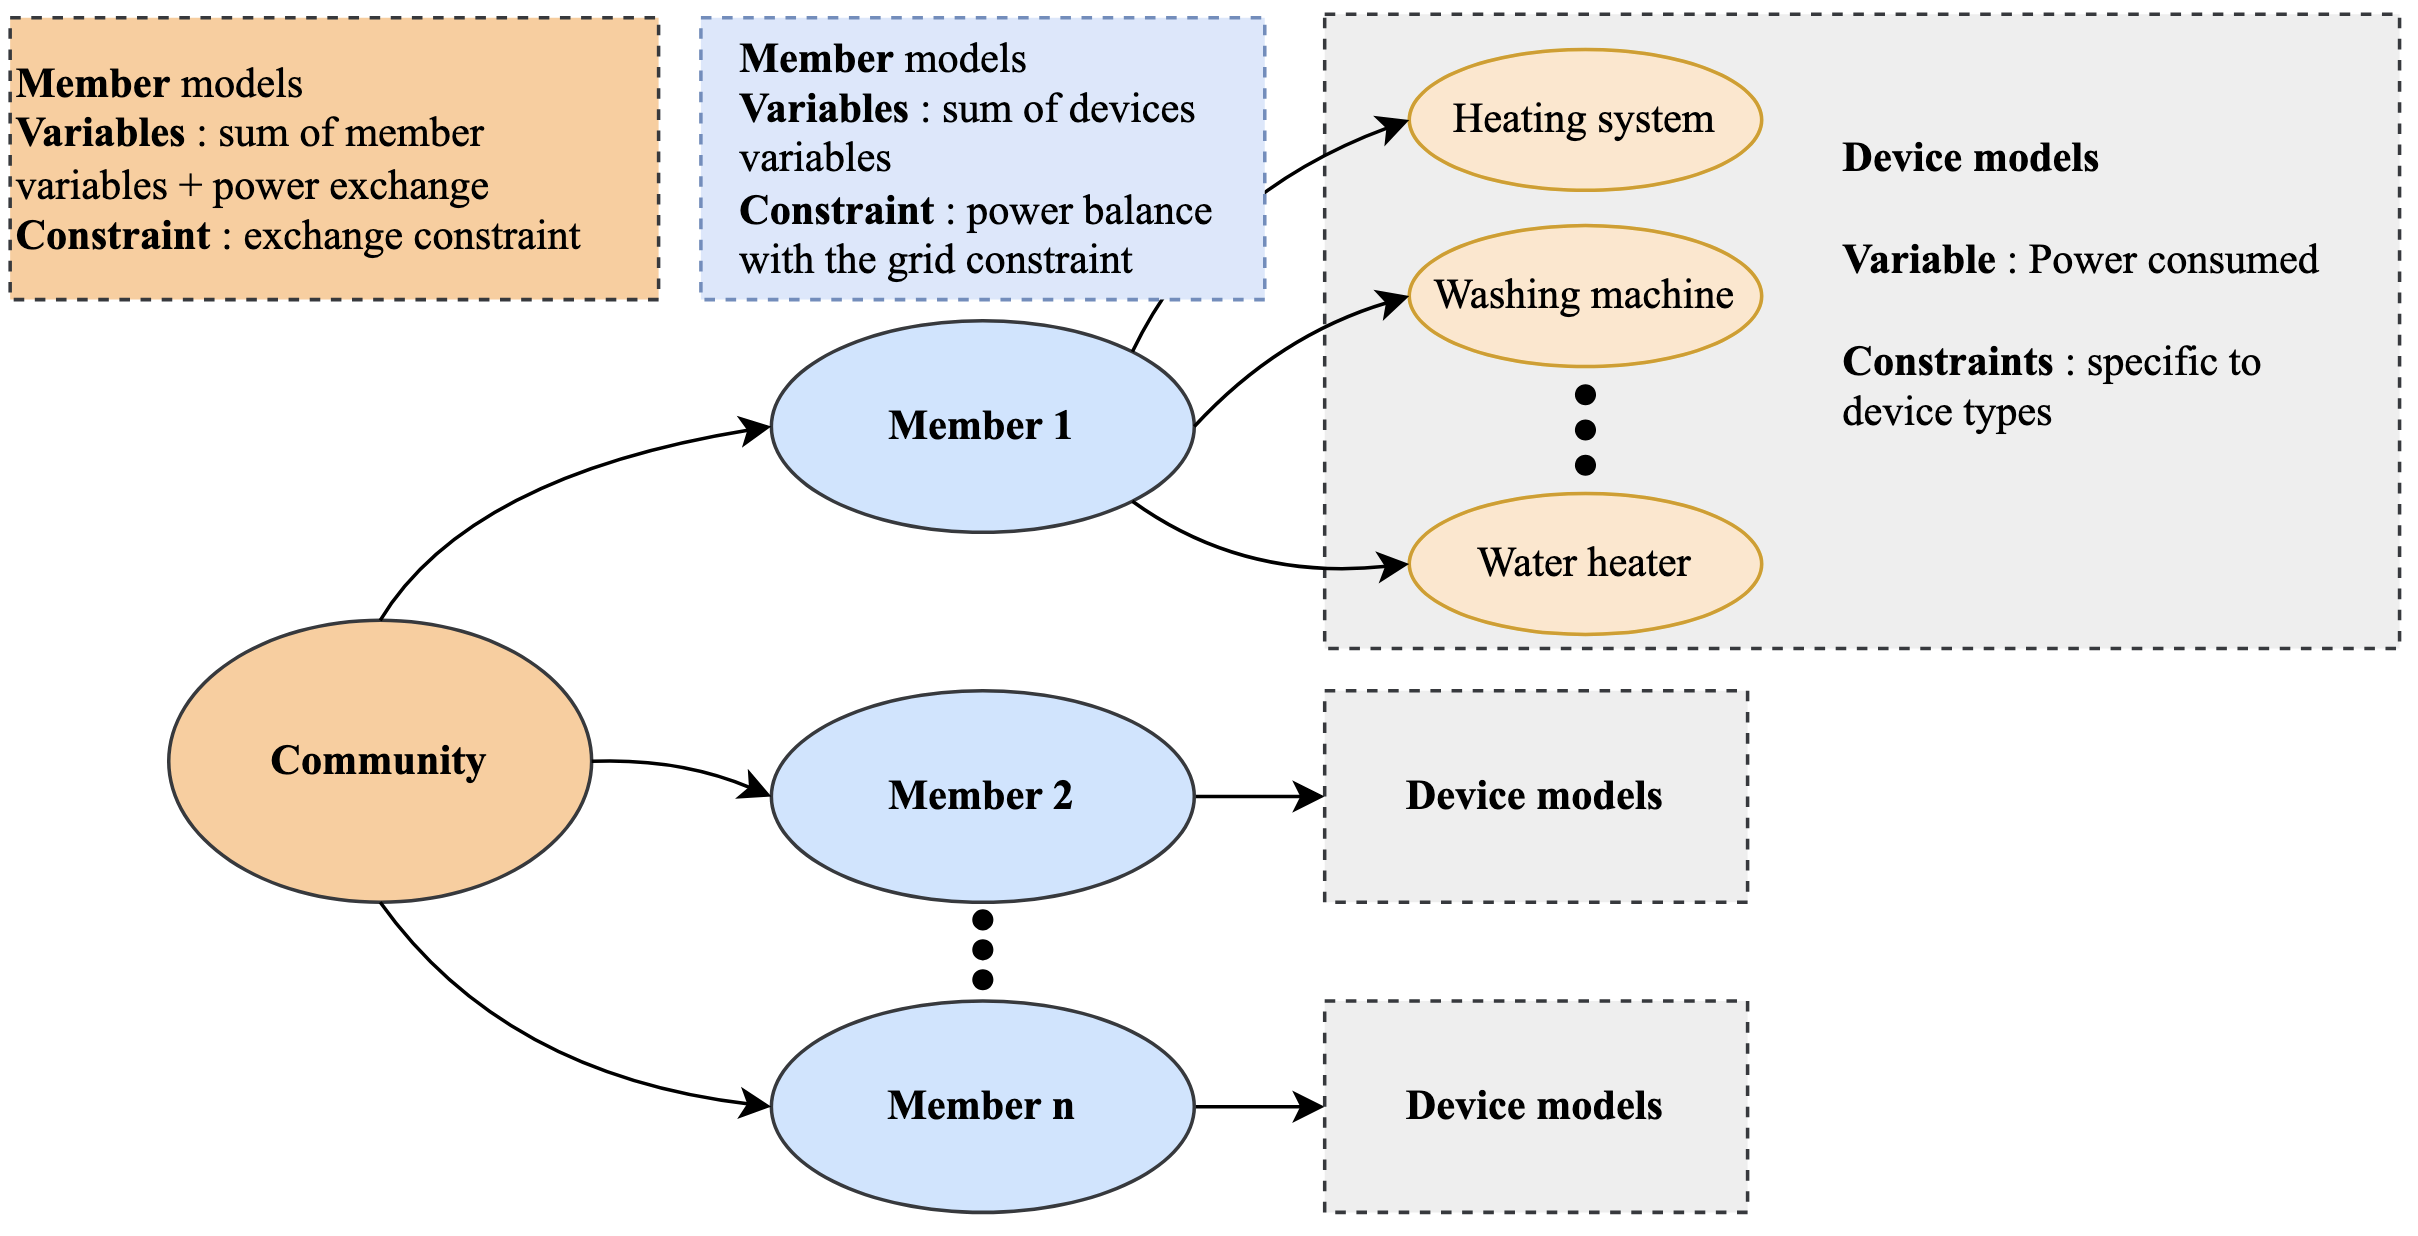
\includegraphics[width=\textwidth]{methodo.png}
    \caption{Model overview}
    \label{fig:methodology}
\end{figure}

\section{Mathematic model}

\subsection{Overview of the models}

As seen in the previous section \ref{methodology}, the model of the community is built in a modular way. We first define the model of the different devices and flexibility services, then the member model and finally the community model. So in this part, we will present in detail how the devices are separated in different categories and how to define their model. Then we will see exactly how the aggregated model are built and define the different objective functions. This model is multi-objective as we want to optimize the community based on sociological profiles of the members. Therefore, we need to build different objective functions, and we need a way to compare them in order to plot the Pareto front.

\subsection{Flexibility services model}

We already identified the different type of flexibility services in the state of the art \ref{section_optimization}. In this work, we will focus on the following ones: the white goods (with a fixed cycle that can be shifted in time), the thermal load (with a comfort range) and the battery storage and electric vehicle (with a storage capacity and a maximum charge and discharge power), and finally the fixed loads with no flexibility.

For each device, what is important is to define one variable representing the consumption profile, that will have the same shape for all the devices, so that they can be summed directly. This variable will be noted $P_{device}$, define as a set of variable for each time step $t \in T$.

\subsubsection{Fixed loads}

Here, the profile is simple enough, the consumption profile is given as a parameter, so the only constraint is  :

\begin{equation} 
    P_{device}[t] = P_{fixed}[t], \forall t \in T
\end{equation}
With $P_{fixed}$ the fixed consumption profile of the device.

\subsubsection{Thermal load}

For defining the thermal load, we have a consumption profile in the form of a range between a minimum and a maximum consumption. We define the maximum consumption as the optimal comfort one. We will then define a variable that compute the gap between the optimal comfort and the chosen power consumption, that will be noted $p_{comfort}$. So we have two constraints defined as follows:
\begin{align} 
    P_{min}[t] \leq P_{device}[t] \leq P_{max}[t], \forall t \in T \\
    p_{comfort}[t] = P_{max}[t] - P_{device}[t], \forall t \in T
\end{align}

\subsubsection{White goods}

For the white goods, we have a fixed cycle that can be shifted in time. So we define a variable 
$x_{start}$ that will be equal to 1 if the cycle starts at time step $t$ and 0 otherwise. This time, we define a comfort time start as well as a time range in which the cycle needs to be executed. Using this, the gap between the starting time and the time wanted ($t_{wanted}$) is defined as a time comfort variable ($t_{comfort}$). In order to use a MILP (mixed integer linear programming) model, we defined two variables in order to define 
$t_{comfort}$, $t_{plus}$ and $t_{minus}$ for positive and negative gap values. 
A parameter $P_{cycle}$ that will be equal to the consumption profile of the cycle is given. For doing so, we define a new time set $T_{cycle}$ that will be all the possible time step of the cycle. The comfort constraints are then defined as follows:


\begin{align}
    &\sum_{t \in T_{cycle}} x_{start}[t] = 1 \\
    &\sum_{t \in T_{cycle}} (t+1) * x_{start}[t] - t_{wanted} \leq t_{plus} \\
    &t_{wanted} - \sum_{t \in T_{cycle}} (t+1) * x_{start}[t] \leq t_{minus} \\
    &t_{comfort} = t_{plus} + t_{minus} 
\end{align}
These constraints ensure that the cycle is executed once and that the comfort time variable is equal to the gap between the wanted time and the actual start time of the cycle.


Then the power consumption constraints are defined as follows:
\begin{align}
    &S_{power}[t] = [max(t-cycle, t_{wanted}-t_{range}), min(t, t_{wanted}+t_{range}-cycle)] \\
    &P_{device}[t] = \sum_{p \in S_{power}[t]} P_{cycle}[t-p] * x_{start}[p], \forall t \in T \\
    &P_{device}[t] = 0, \forall t \notin T_{cycle} 
\end{align}
With $cycle$ being the duration of the cycle. These power constraints ensure that the power consumption of the device is equal to the cycle profile when the cycle is running and 0 otherwise.

\subsubsection{Battery storage and electric vehicle}

Finally, comes the battery storage and electric vehicle. The only difference between the two is that we cannot operate the electric vehicle when it is not at home. Also, a minimum state of charge is required before leaving and a new value is defined after coming back home. The choice has been to define a battery as a fixed electric vehicle, so both of them have the same constraints. Here are the constraints for the battery storage and electric vehicle:

        
\begin{align}
    &E[t] = E[t-1] + P_{plus}[t] * \eta_{charge} - P_{minus}[t] / \eta_{dcharge}, \forall t \in T_{Home} \\
    &P_{device}[t] = P_{plus}[t] - P_{minus}[t], \forall t \in T_{Home} \\
    &P_{device}[t] = 0, \forall t \in T_{NotHome} \\
    &E[0] = E_0 \\
    &E[end] = E_{end} \\
    &E[t] \geq E_{min}[t], \forall t \in T_{leave} \\
    &E[t] = E[t'] - \Delta E, \forall t \in T_{back} \text{ and } t' \text{equal to the corresponding leave time}
\end{align}
With $E$ the state of charge of the battery, $P_{plus}$ and $P_{minus}$ the charge and discharge power. They are here to differentiate between the charging and discharging phase. Those values are positive. $\eta_{charge}$ and $\eta_{dcharge}$ the charge and discharge efficiency, $E_0$ the initial state of charge, $E_{end}$ the final state of charge. $E_{min}$ is the list of the minimum state of charge at the different leave time, $\Delta E$ is the energy needed for the trip and $T_{leave}$ and $T_{back}$ are the time steps of leaving and coming back home. Finally, $T_{Home}$ and $T_{NotHome}$ are the time steps when the electric vehicle is at home or not respectively. 

\subsection{Prosumer model}

Each member of the community is defined as a prosumer, meaning that they can both produce and consume energy. Their consumption profile is defined by the different devices they have, while their production profile is given as a parameter. This model supposes that we know beforehand the production profile of each member, by a predicting model for example. We then need to add to the model the power exchange with the community and with the grid.

The first step here is to define the link between the different devices and the total consumption profile of the member. This is done by defining a variable $P_{member}$ and $P_{battery}$ this way : 

\begin{align}
    &P_{member}[t] = \sum_{d \in D} P_{d}[t], \forall t \in T \\ 
    &P_{battery}[t] = \sum_{d \in D_{battery}} P_{d}[t], \forall t \in T
\end{align}
With $D$ the set of devices of the member other than the battery storage and electric vehicle, and $D_{battery}$ the set of battery storage and electric vehicle devices.

For the power exchange with the community, we will differentiate between the power coming from the community and the power sent to the community. Also, we enable exchanges within the community only from the produced energy, coming either from the power source or from the battery storage. For doing so, again we need to define a positive and negative variable for the battery power ($P_{bat+}$ and $P_{bat-}$). So we define a variable $P_{shared}$ and a variable $P_{self}$ for the shared and self-consumed power respectively. The constraints for sharing power are defined as follows:

\begin{equation}
    P_{shared}[t] + P_{self}[t] = P_{prod}[t] + P_{bat-}[t], \forall t \in T
\end{equation}

At the member scale, we will not consider in the power balance the power sent to the community, as it will be done at the community level. So for the power balance we consider only the power coming from the community defined as $P_{received}$. For the power exchanged with the grid, we want to differentiate between the power bought from the grid and the power sold to the grid for the objective function definition. So we define two variables $P_{grid+}$ and $P_{grid-}$ for the power bought and sold to the grid respectively. The power balance constraint is defined as follows:
\begin{equation}
    P_{grid+}[t] - P_{grid-}[t] = P_{member}[t] + P_{bat+}[t] - P_{received}[t] - P_{self}[t], \forall t \in T
\end{equation}
We can also sum the comfort variables of the different devices to have a global comfort variable for the member.

By adding the objective functions to this model, we can complete the fully decentralized optimization model. These objective functions will be defined just after in \ref{objective_function}.

\subsection{Community model}
The community model is built by aggregating the different member models and adding the constraints related to the power exchange between the members. For doing so, we need to define a variable $P_{exchange}[i, j, t]$ for each time step $t$ and each pair of members $i$ and $j$. It represents the power sent from member $i$ to member $j$ at time step $t$ and is positive. The power balance constraints for the community are then defined as follows: 

\begin{align}
    &P_{received, m}[t] = \sum_{j \in M} P_{exchange}[j, m, t], \forall m \in M, \forall t \in T \\
    &P_{exchange}[i, i, t] = 0, \forall i \in M, \forall t \in T 
\end{align}
With $M$ the set of members of the community. The power consumed, produced as well as the comfort variables can then be summed directly from the member models. By adding an objective function to this model, we can optimize the system in a fully centralized way.

\subsection{Objective function definition}
\label{objective_function}

In \cite{these_sorel}, they use a vector of the sociological profile of each member of the community in order to define a multi-objective optimization problem as explained in the state of the art \ref{section_sociological_profiles}. In this work, we reproduced this idea. They used a vector of 3 dimensions, the economic dimension, the environmental dimension and the independence dimension.

The way the model is built here, the independence dimension is linked very strongly to the other two dimensions, that already try to maximize the self-consumption of the members. Furthermore, the flexibility could very well impact the comfort of the members. So the idea has been to replace the independence dimension by a comfort dimension. The independence dimension could be more interesting in a model as defined in \cite{article_5} where the community become disconnected from the main grid.

For the economic dimension, it is easy to define the objective function as the cost of the energy bought from the grid minus the revenue from the energy sold to the grid. For the environmental dimension, we can associate to the grid energy a carbon footprint and another one to the energy consumed by the devices. For example, in France, the carbon footprint of the grid energy is in average equal to 40 gCO2/kWh in 2022 while for the same year, in France, the carbon footprint of the energy produced by a PV panel is around 25 gCO2/kWh. Of course a more accurate study could be done by looking exactly at the installation of each member of the community. The main point is that the two objective functions defined like this will remain linear and that we could imagine some coefficient to be able to compare the two dimensions easily. Here are the equations of such objective functions :

\begin{align}
    ElectricityPrice = \sum_{t \in T} &\big(P_{grid+}[t] \cdot BuyPrice[t] - P_{grid-}[t] \cdot SellPrice[t] 
        \nonumber \\&+ P_{received} \cdot CommunityPrice\big)  \\ \nonumber \\
    CarbonFootprint = \sum_{t \in T} &\big(P_{grid+}[t] \cdot GridFootprint[t] \nonumber \\
    &+ P_{self}[t] \cdot SelfFootprint 
        \nonumber\\
        &+ P_{shared}[t] \cdot SharedFootprint\big)
\end{align}
With $BuyPrice$ and $SellPrice$ the price of buying and selling energy to the grid, $CommunityPrice$ the price of energy received from the community, $GridFootprint$, $SelfFootprint$, and $SharedFootprint$ the carbon footprint of the grid energy, the self-consumed energy, and the shared energy respectively. For simplicity's sake, the prices and carbon footprint have been considered as constant over time. In this study we took $CommunityPrice$ equal to 0. But this number could be used to study the effect of dynamic pricing within the community for example.


But for the comfort, we have the choice about how to build the objective function, and it seems to be harder to compare with the other. The choice made in this work is to make a linear objective function, and then we will compute before each optimization references value of the community (or the member) for each dimension. We will then divide the value of the objective function by this reference value in order to pass in per unit values and be able to compare the objective functions. So here is the equation of the comfort objective function:

\begin{equation}
    Comfort = \sum_{t \in T} p_{comfort}[t] \cdot coef_p + t_{comfort} \cdot coef_t \cdot |T|
\end{equation}
With $coef_p$ and $coef_t$ the coefficient for the power comfort and time comfort respectively. The choice of these coefficients will determine the importance of each term in the comfort objective function. For this study they have been set to 1 each.

Finally the complete objective function is defined as follows:

\begin{equation}
    Objective = w_{eco} \cdot \frac{ElectricityPrice}{ref_{eco}} + w_{env} \cdot \frac{CarbonFootprint}{ref_{env}} + w_{comfort} \cdot \frac{Comfort}{ref_{comfort}}
\end{equation}
With $w_{eco}$, $w_{env}$, and $w_{comfort}$ the weight of the economic, environmental, and comfort dimension respectively. $ref_{eco}$, $ref_{env}$, and $ref_{comfort}$ the reference value for the economic, environmental, and comfort dimension respectively.

For defining the reference value, we need to be able to compute the value of each objective function in the exact same condition. So we will need to define a basic case that will serve to evaluate the reference value for each dimension. In this case, we considered a medium comfort case with no exchanges and use of the battery storage. Which mean that the consumption profile of each member is the one defined by the devices, and when the devices have a flexibility range, we place ourselves in the middle of this range. Defined like this, we will be able to compute a Pareto front of the model by changing the weight of the different dimensions in the objective function. 

The full optimization model is a mixed integer linear programming (MILP) model, as we have binary variables for the white goods and continuous variables for the other devices. The optimization is done using the Python library Pyomo and the solver used is Gurobi.

\section{Gains allocation}

\subsection{Gain allocation functions}

At this stage, we have a model that let us operates the community in a fully centralized way as well as in a fully decentralized way. This way we can compute the gain of the community by comparing the cost of the community in the centralized case with the cost of the community in the decentralized case. As the model in the centralized case hold more information and does not add constraints that will affect the objective cost negatively, we can be sure that the cost of the community in the centralized case will be lower than the cost of the community in the decentralized case. Thus, we can be sure that the gain of the community will be positive. We can then define a gain allocation vector $x$ that will give to each member of the community a share of the gain. So we should have :
\begin{align}
    &Gain = Objective_{centralized} - \sum_{i \in M} Objective_{centralized,i} \\
    &\sum_{i \in M} x_i = Gain
\end{align}
With M the set of members of the community, $Objective_{centralized}$ the value of the objective function in the centralized case, and $Objective_{centralized,i}$ the value of the objective function for member i in the centralized case.

For this, we will use the functions defined in the state of the art section \ref{section_allocation}. As said in \ref{methodology}, we will use the Shapley value defined in equation \ref{eq:shapley}, the proportional allocation defined in equation \ref{eq:PA}, and an egalitarian allocation defined as follows:
\begin{equation}
    x_i = \frac{Gain}{|M|}
\end{equation}
With $|M|$ the number of members in the community. 

Of course, it does not make sense to allocate environmental gains or comfort gains without changing the operation of the community. So when allocating the gains, we will only talk about the economic gains. But we can still compute the proportional allocation and Shapley value using the total objective gain in order to consider the contribution of each member for the total objective of the community.

The full optimization process is shown in figure \ref{fig:gain_allocation}. 

\begin{figure}[ht]
    \centering
    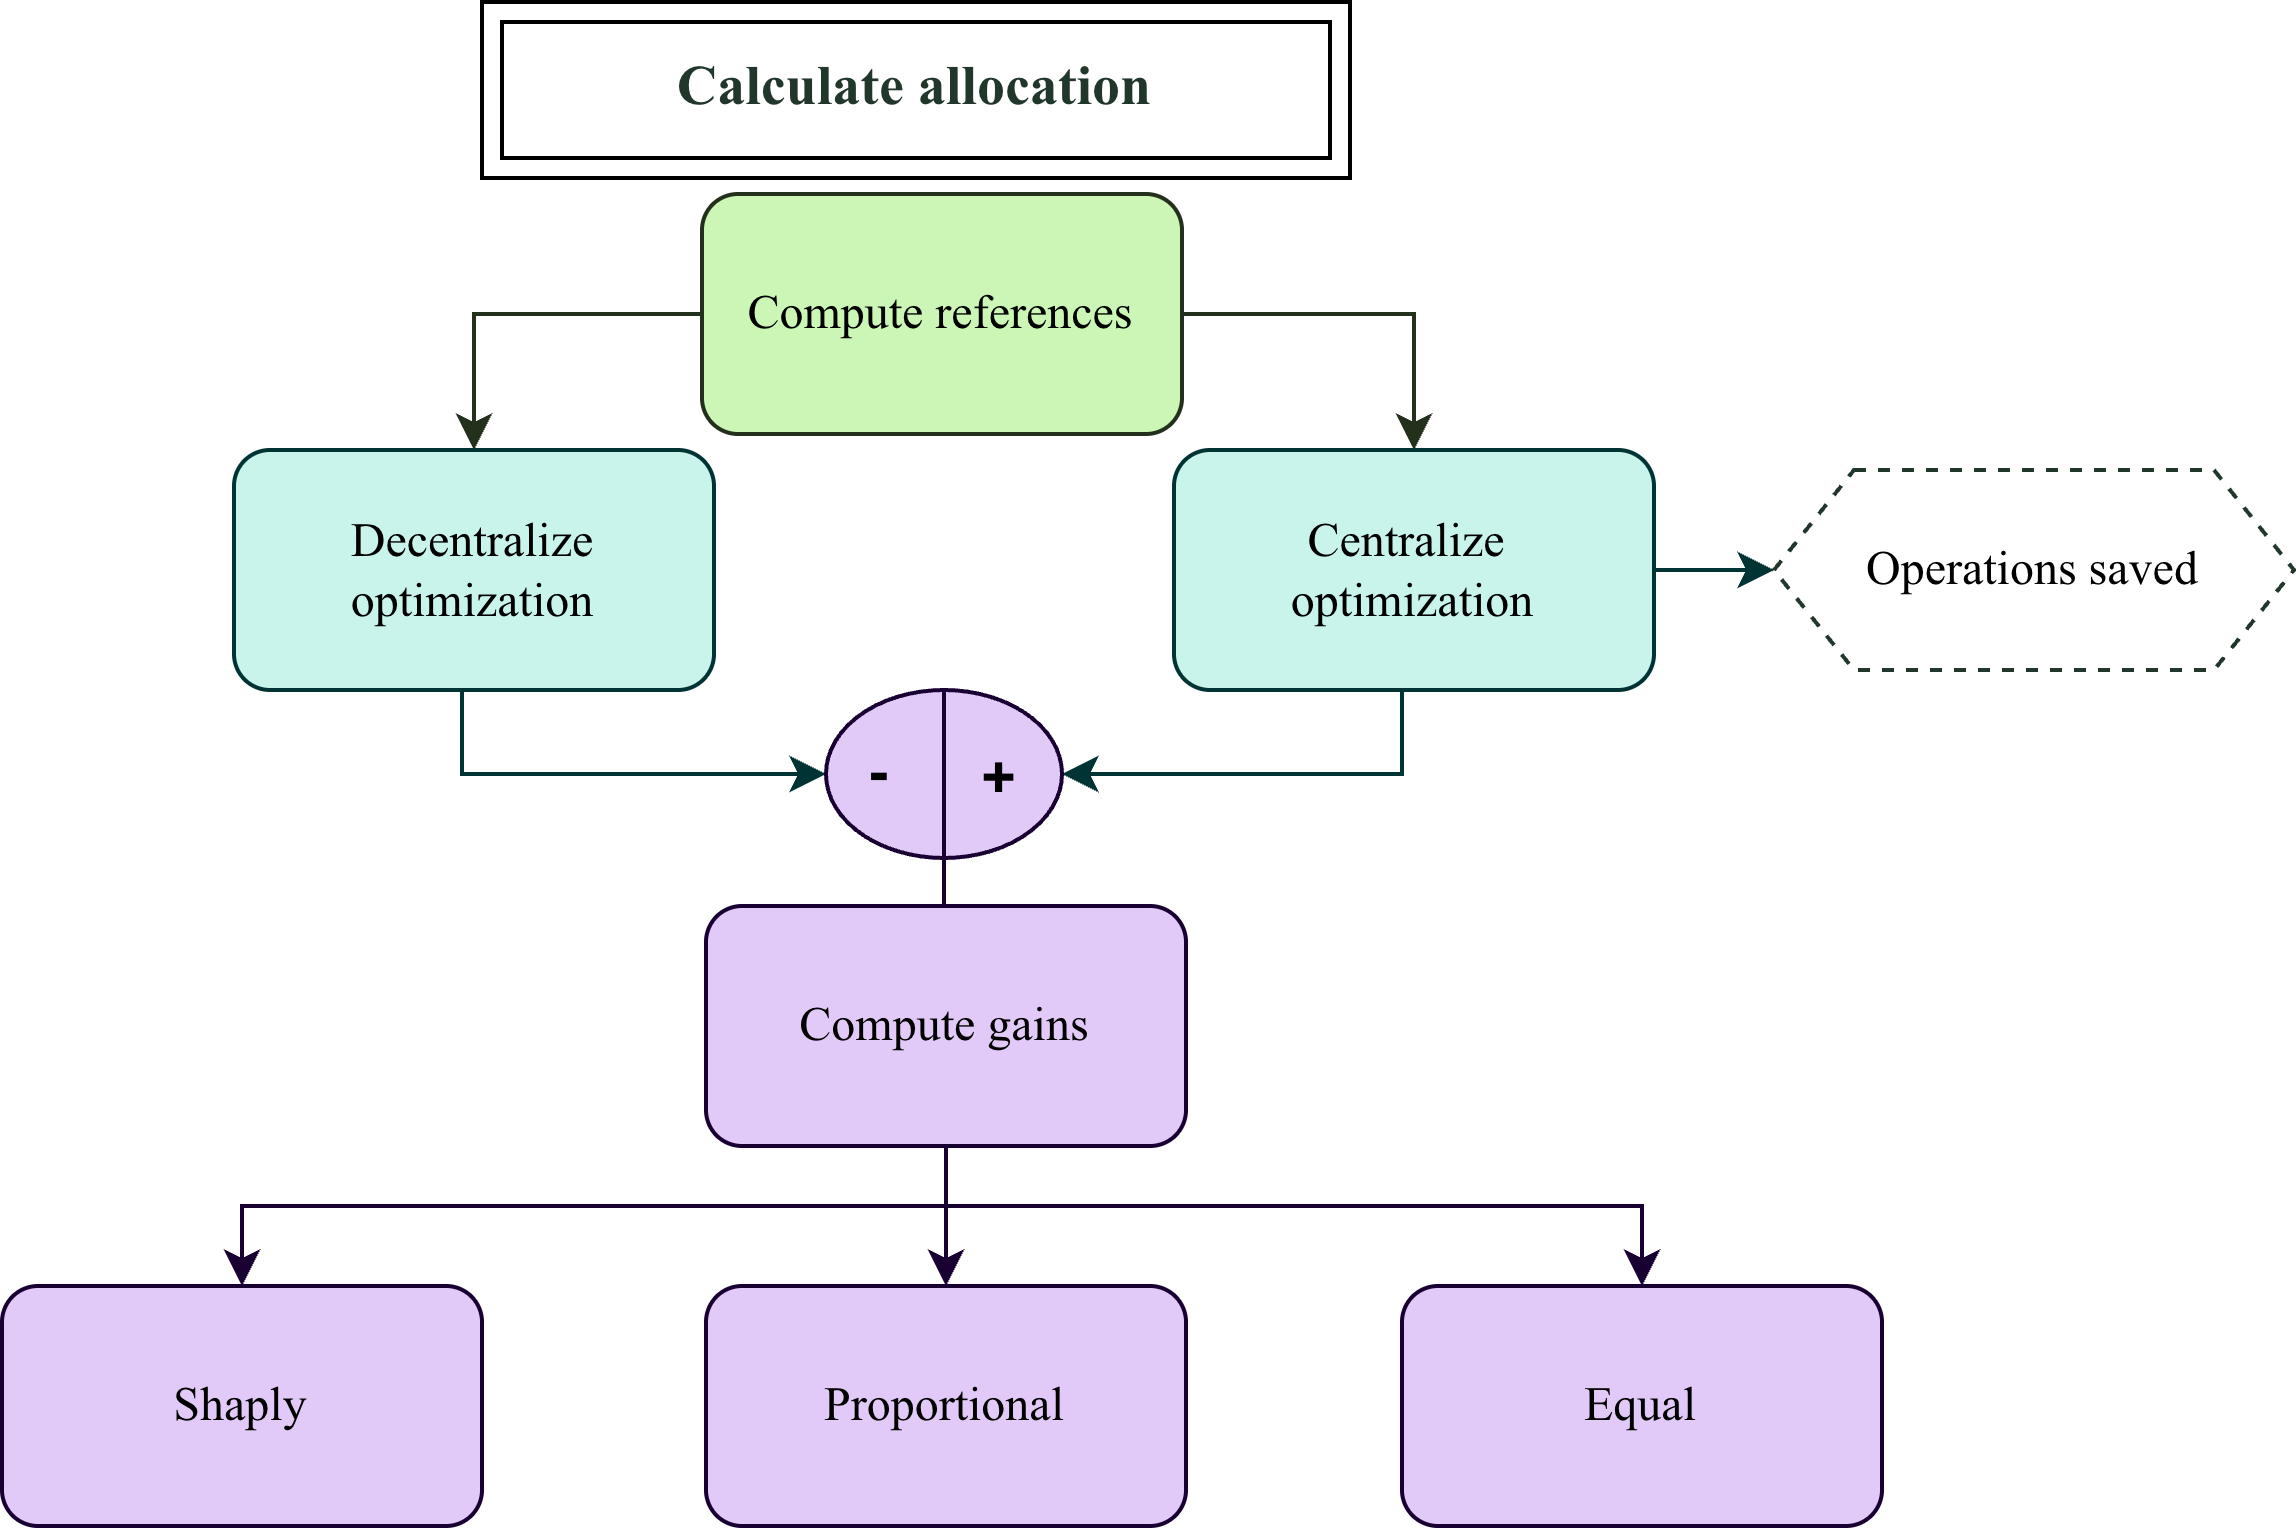
\includegraphics[width=0.6\textwidth]{allocation_schema.png}
    \caption{Gain allocation process}
    \label{fig:gain_allocation}
\end{figure}


\section{Results}

\subsection{Verification of the model}

When adding different members with a lot of different devices, the model can become quite complex. Thus, it becomes impossible to verify if the behaviors observed are the expected ones. So before trying to make any results, a set of tests were made to verify that the model of each device works as expected.

\begin{table}[h!]
    \centering
    \begin{tabular}{|c|c|c|c|}
        \hline
        Member & Heating system (thermal load) & Washing machine (white good) & Electric vehicle \\ \hline
        1      & X  &    &    \\ \hline
        2      &   & X &     \\ \hline
        3      &   &  & X   \\ \hline
        4      & X   & X  & X   \\ \hline
    \end{tabular}
    \caption{Members test setup}
    \label{tab:test_members}
\end{table}

The table \ref{tab:test_members} shows the setup of each member in terms of devices. The presence of an "X" in a cell indicates that the corresponding device is present for that member. This way, by putting a production between 10AM and 2PM, we should see that the electric vehicle is charged during this period for member 3, that the washing machine is used during this period for member 2, and that the heating system is used more strongly during this period with sociological profiles of ["economic" : 1, "environmental" : 0, "comfort" : 0.1] (in the following parts, the profiles will be noted as [economic, environmental, comfort], so here it would be [1, 0, 0.1]).

Another test was made to verify the model for the exchanges between the members. For this, we made a community with 2 members, one with a production profile constant equal to 10 and the other without. Both of them have a fixed load of 5. As the selling price is lower than the buying price, with a none 0 coefficient for the economic dimension, we should see that the first member sell its excess production to the second member and not to the grid.

Using these tests, we are able to verify that the model works as expected.

\subsection{Construction of the example}

In order to produce results, an example was built. In this example, we defined the parameters of several devices based on very simple physic models and average power output of the different elements. For example, the power of the heating system is linear with the difference between the indoor and outdoor temperature and comparing to real power consumption figures from a bill we can get a power output of around 100 W/°C. The same was done for other devices. For the production profile, we used an irradiance profile built using PVGIS in December at Villeneuve d'Ascq. 

Then based on a presence at home profile, we can define rules for the consumption of the different devices. If we take again the heating system, when the person is at home, the heating system have a maximum comfort reference temperature which depend on the member. Here this reference can vary between 19 and 22 °C. While when the person is not at home, the heating system have a maximum temperature of 15 °C. This gives a reference consumption profile for the heating system. For the possibility of providing flexibility services, we also define a minimum temperature for when the person is at home (here 18 °C). Of course some devices do not have any flexibility range, for example, the lights are on when the person is at home and it is night, and they are off otherwise.

As shown in \ref{fig:methodo_example}, a function that generate random profiles and a function that allocate to a member different devices randomly were built. This way we can easily generate different examples with different production and consumption profiles. Then, the more fitted members can be chosen to build a community where the optimization will be more interesting. Indeed, if the production profiles is always below the consumption profile, the optimization will not be very interesting as the community will not be able to share energy. The other way around, if every member has a high production and battery storage, then sharing energy will not be useful neither.

\begin{figure}[h]
    \centering
    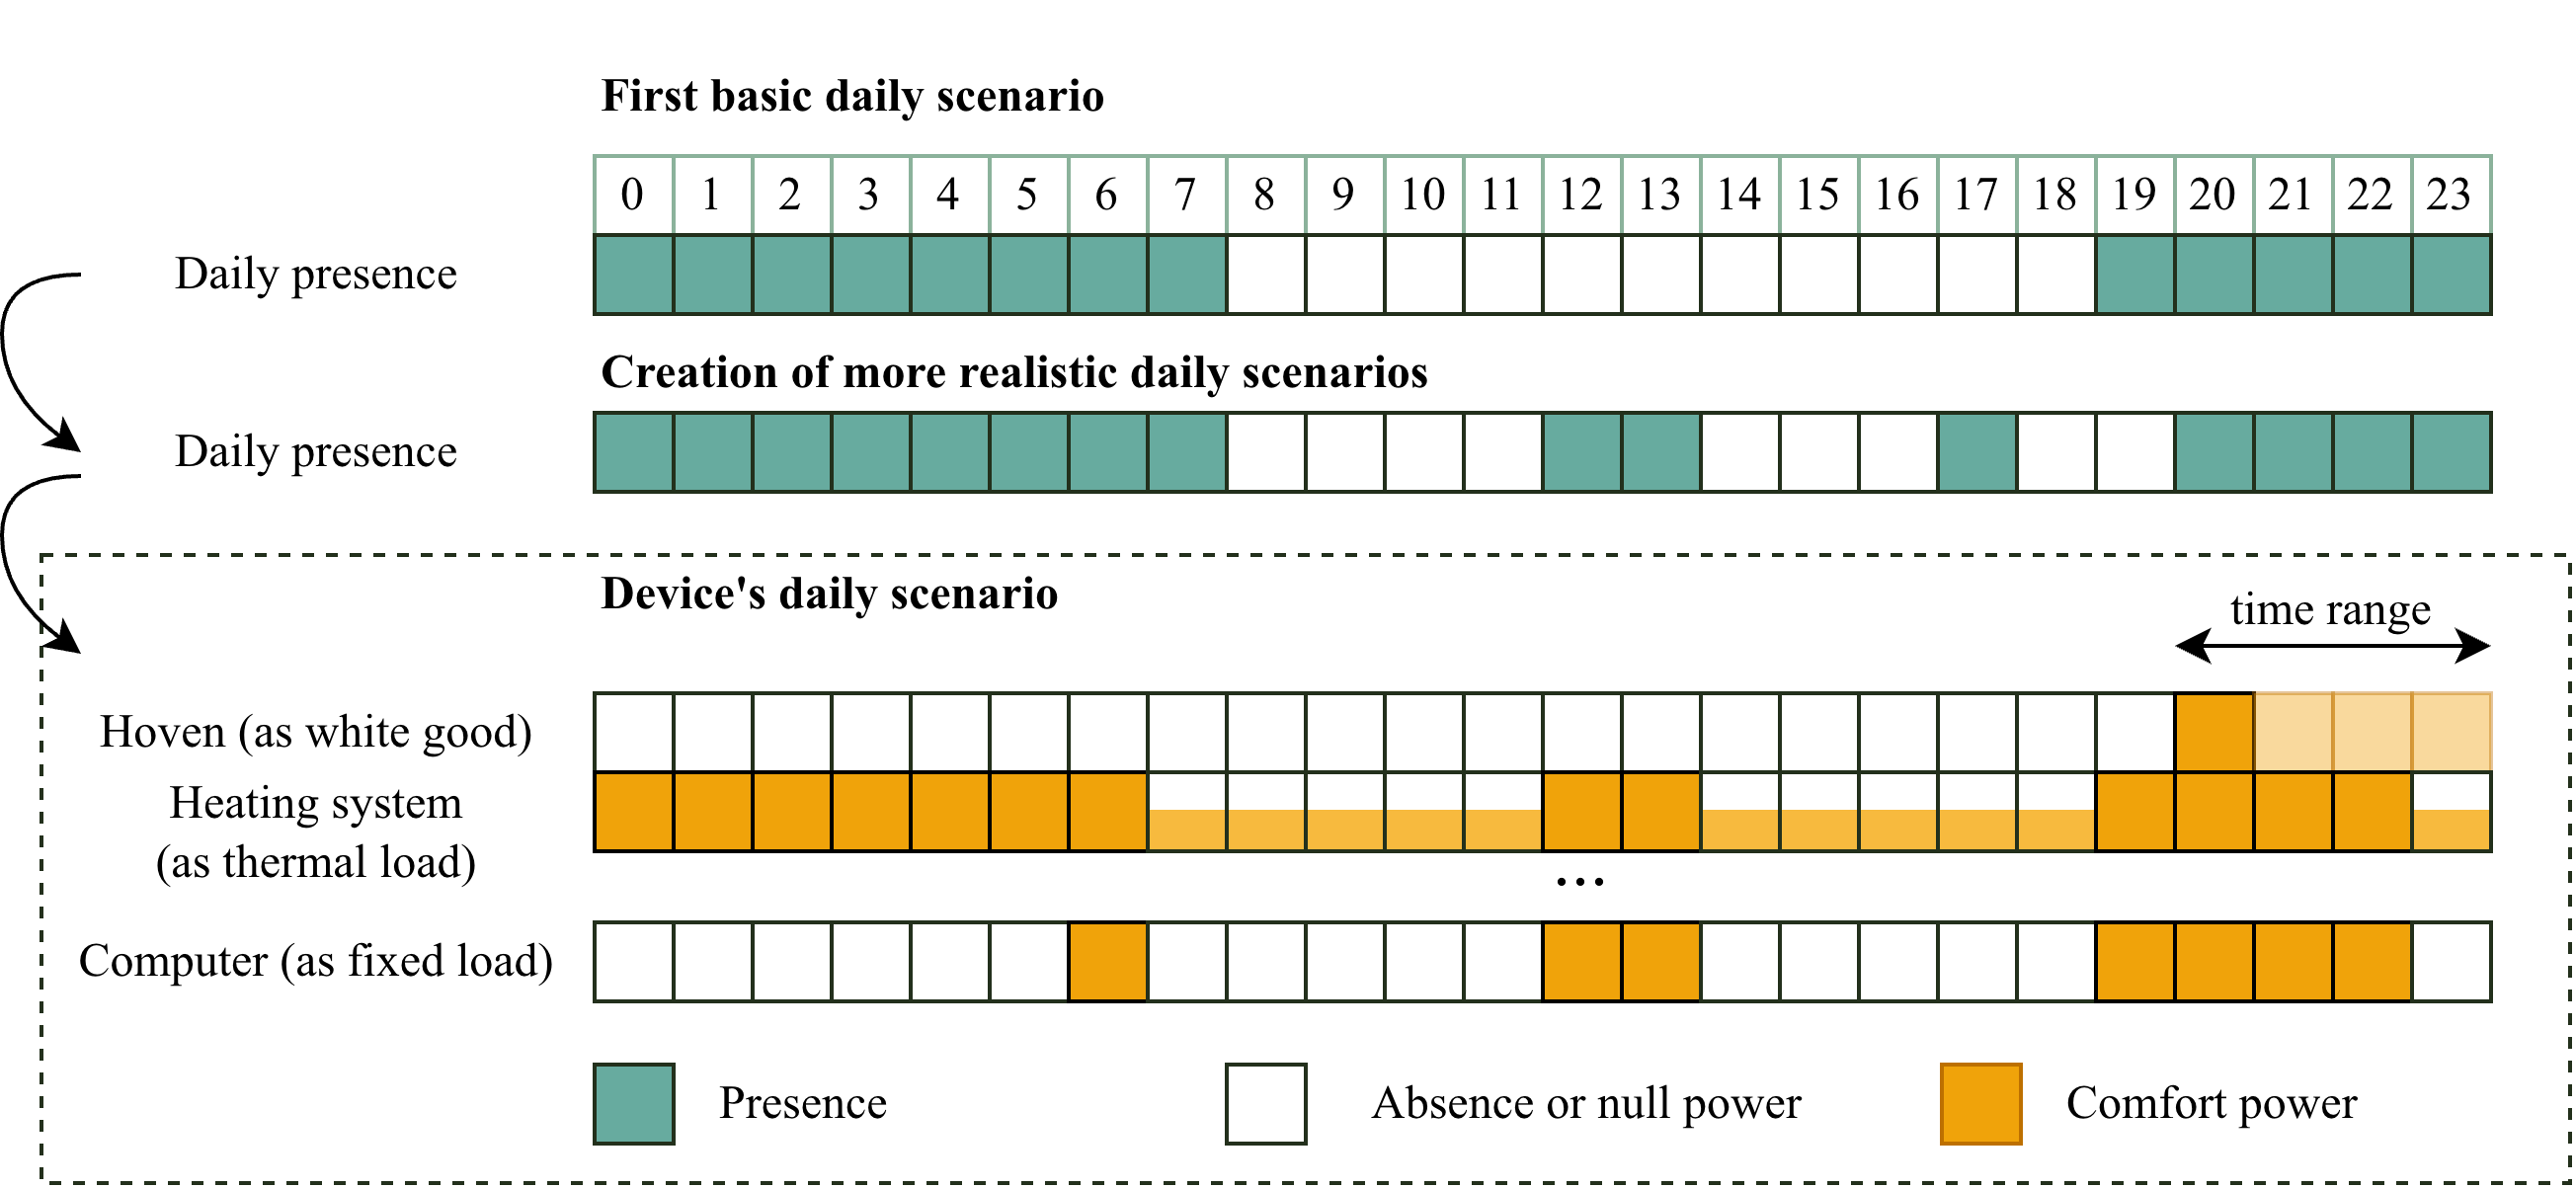
\includegraphics[width=0.7\textwidth]{creation_example.png}
    \caption{Example generation process}
    \label{fig:methodo_example}
\end{figure}

In the end, the community is made of 5 members, so that the results will remain easy to read. The table \ref{fig:table_example} gives the setup of each member of the community in terms of devices. We will then define the sociological profiles based on what we want to show in the different visualizations. Figure \ref{fig:power_profiles_example} shows the power profiles of the different members of the community, for this there are optimized in a fully decentralized way with a sociological profile of [1, 1, 1] for all the members. 


\begin{figure}[!h]
    \centering
    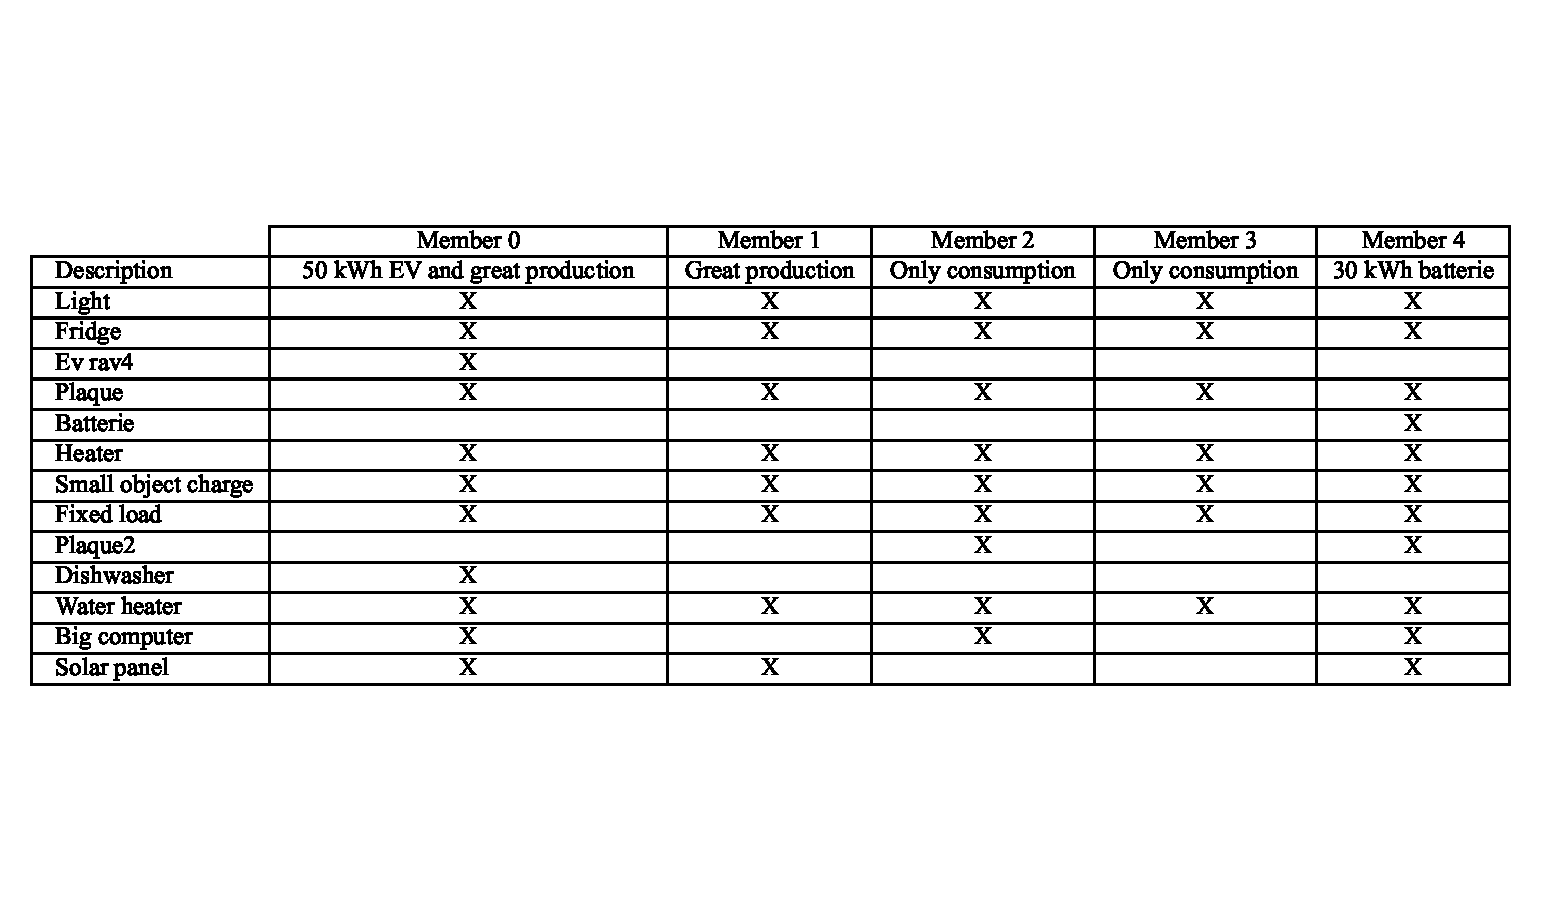
\includegraphics[clip, trim=0cm 4cm 0cm 4cm, width=\textwidth]{dataframe_output.eps}
    \caption{Example setup}
    \label{fig:table_example}
\end{figure}

\newlength{\subfigwidth}
\setlength{\subfigwidth}{0.32\textwidth}
\begin{figure}[h]
    \centering
    \begin{subfigure}[b]{\subfigwidth}
        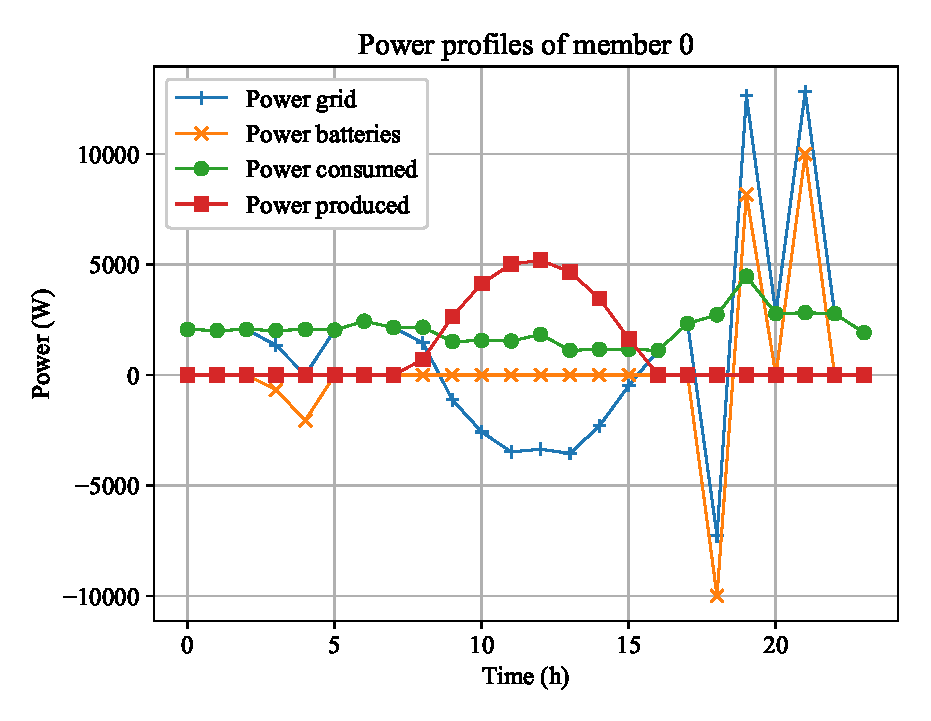
\includegraphics[width=\textwidth]{member_profiles/member_0_power_profiles.eps}
    \end{subfigure}
    \begin{subfigure}[b]{\subfigwidth}
        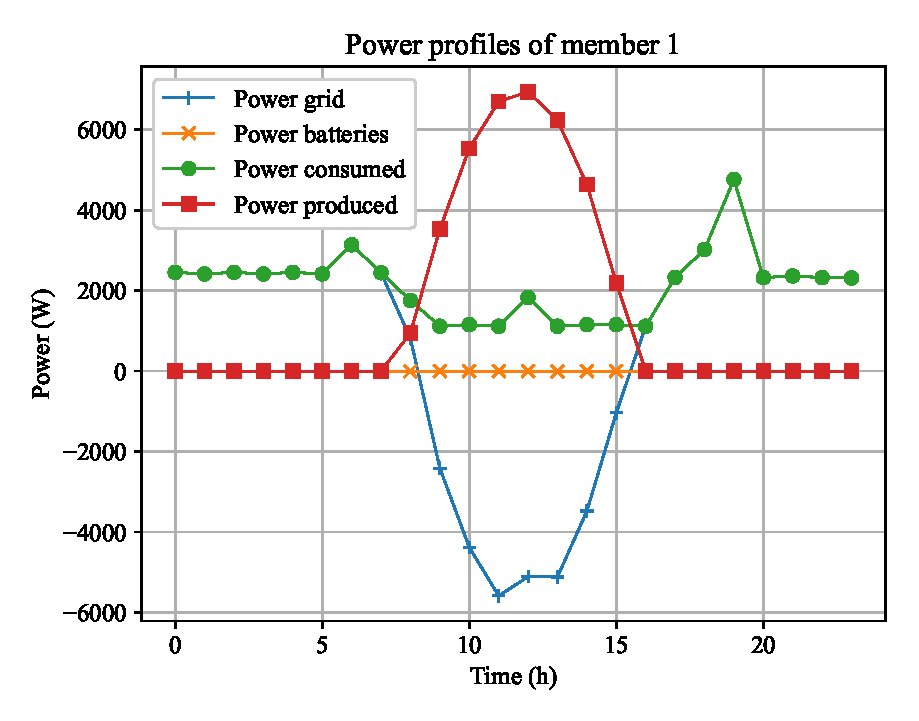
\includegraphics[width=\textwidth]{member_profiles/member_1_power_profiles.eps}
    \end{subfigure}
    \begin{subfigure}[b]{\subfigwidth}
        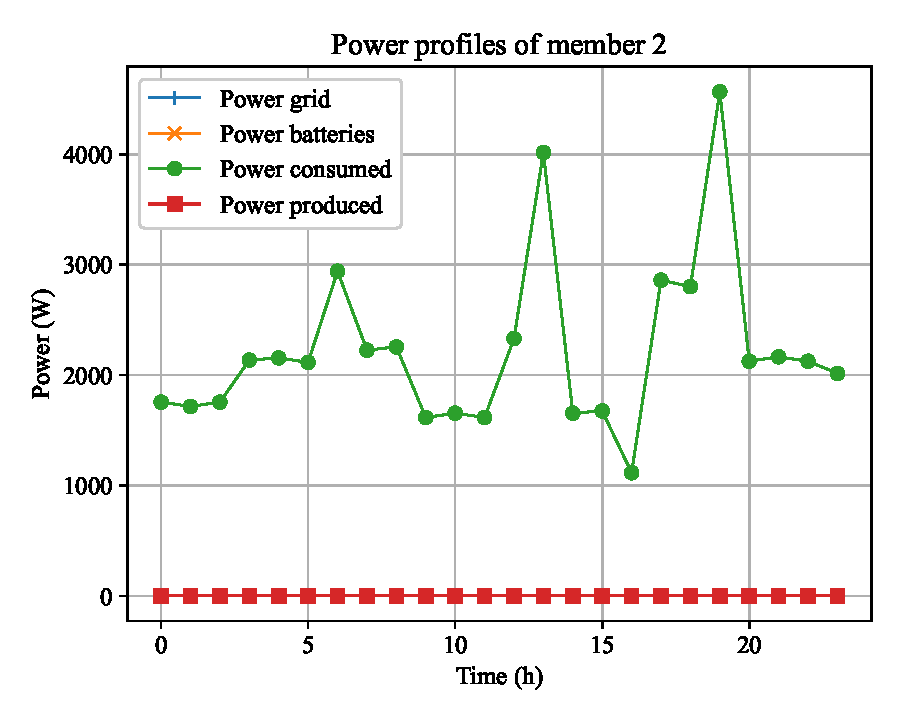
\includegraphics[width=\textwidth]{member_profiles/member_2_power_profiles.eps}
    \end{subfigure}
    \begin{subfigure}[b]{\subfigwidth}
        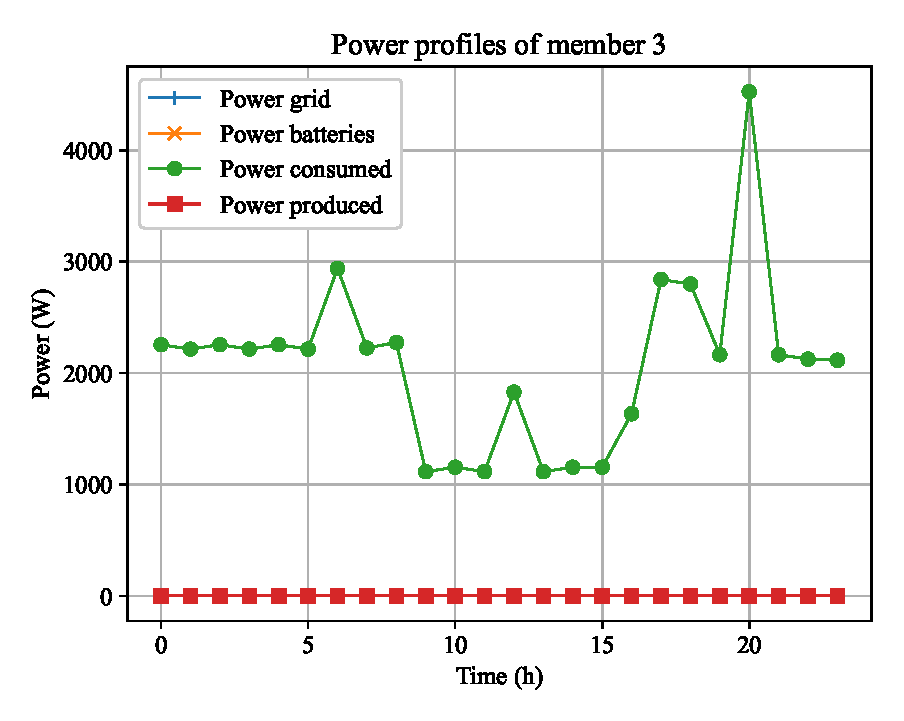
\includegraphics[width=\textwidth]{member_profiles/member_3_power_profiles.eps}
    \end{subfigure}
    \begin{subfigure}[b]{\subfigwidth}
        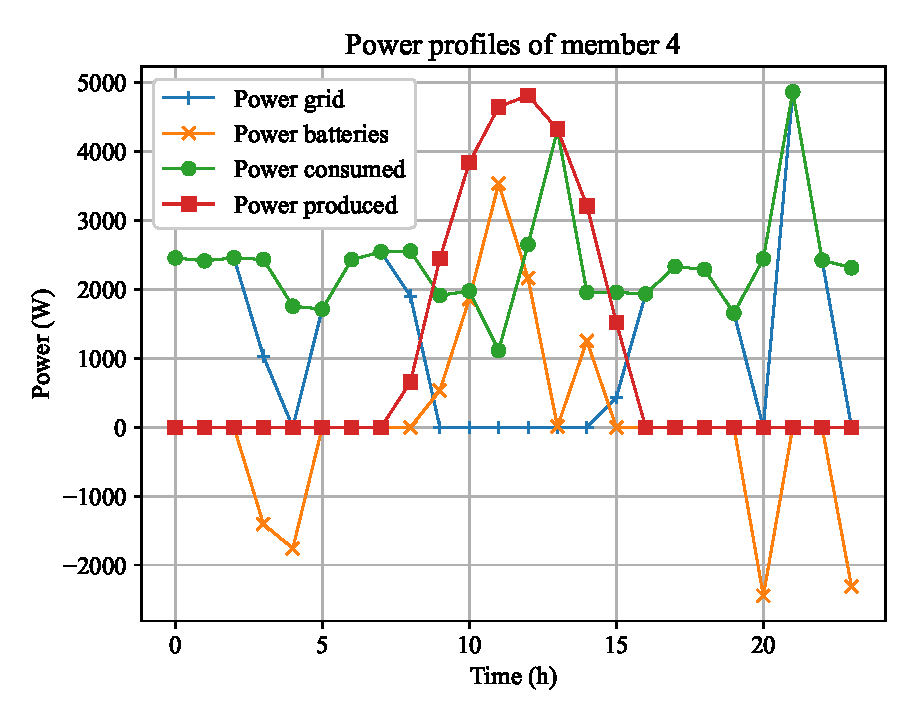
\includegraphics[width=\textwidth]{member_profiles/member_4_power_profiles.eps}
    \end{subfigure}
    \caption{Profile of each member when optimized in a fully decentralized way with a sociological profile of [1, 1, 1] for all the members.}
    \label{fig:power_profiles_example}
\end{figure}
\subsection{Optimization of the community}

With the model of the community built, we can first launch the optimization in a fully decentralized way with a sociological profile equal to [1, 1, 1] for all the members just to look at the behavior of the system. Figure \ref{fig:community_centralized} shows that at midday, the production being a lot higher than the consumption, there is a lot more exchanges withing the community and the batteries are charging. Outside of this, it is quite hard to understand specifically what is happening. Though, we can compare it with the operation when we have different sociological profiles. Figure \ref{fig:diff_profiles} shows the operation of the community with a sociological profile of [1, 0, 0], [0, 1, 0] and [0, 0, 1] for all the members. We can see here, that between the economic only profile and the environmental only one there are some differences, but still, they are quite similar. With the comfort only profile, the model does not care about the community and just maximize the consumption at the wanted time and power output. But it is still hard to interpret what will be the effect of the sociological profile on the operation.

\begin{figure}[!h]
    \centering
    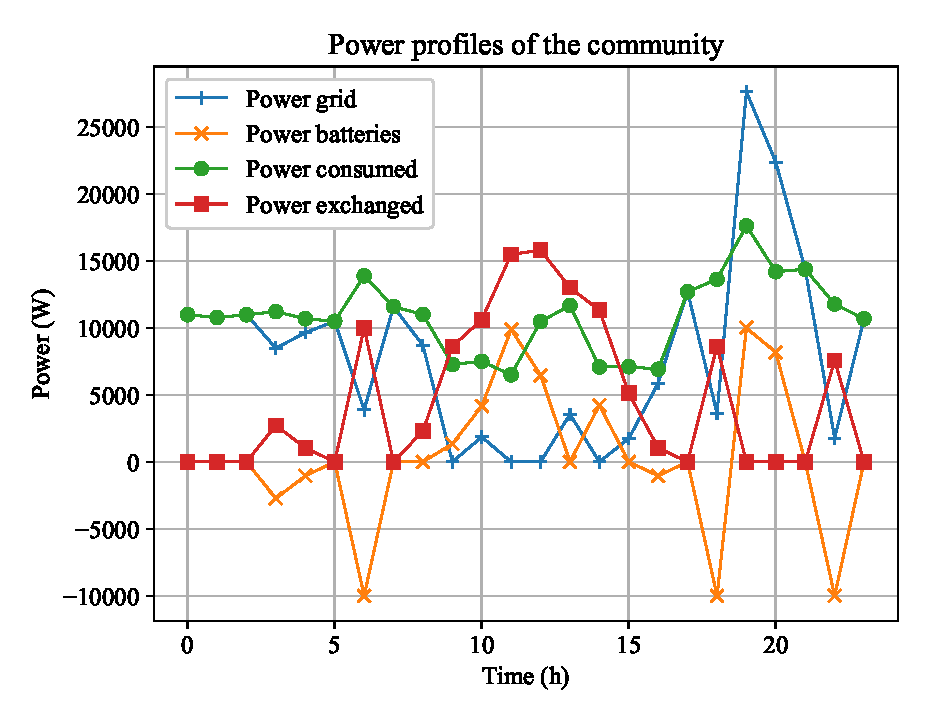
\includegraphics[width=0.48\textwidth]{community_centralized.eps}
    \caption{Operation of the community optimized in a fully centralized way with a sociological profile of [1, 1, 1] for all the members.}
    \label{fig:community_centralized}
\end{figure}

\begin{figure}[!h]
    \centering
    \begin{subfigure}[b]{0.32\textwidth}
        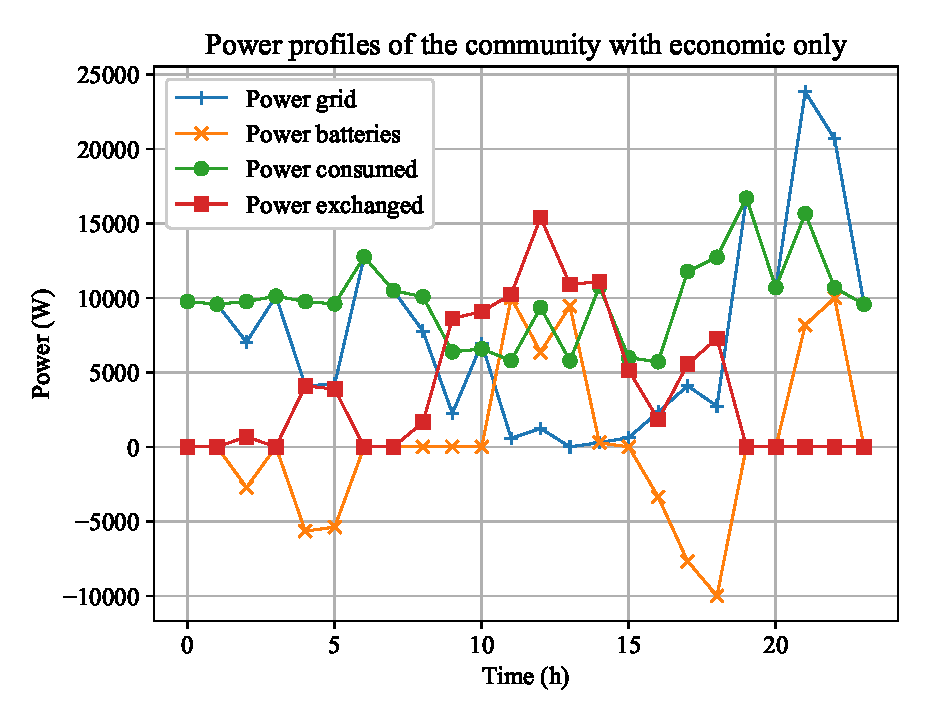
\includegraphics[width=\textwidth]{community_profiles/community_economic_only_power_profiles.eps}
        \caption{Sociological profile [1, 0, 0]}
    \end{subfigure}
    \begin{subfigure}[b]{0.32\textwidth}
        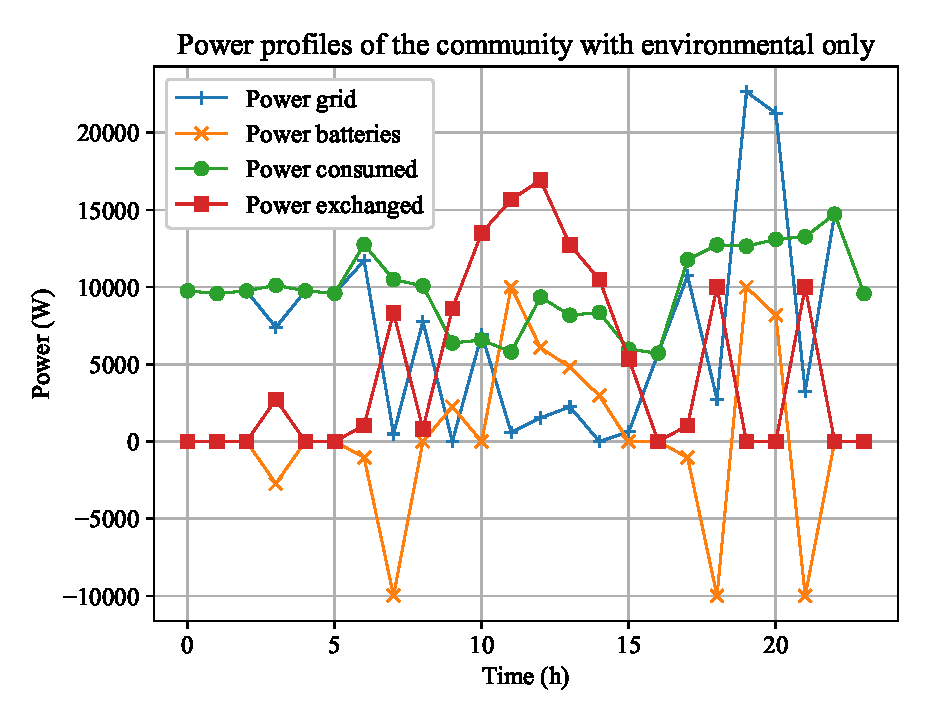
\includegraphics[width=\textwidth]{community_profiles/community_environmental_only_power_profiles.eps}
        \caption{Sociological profile [0, 1, 0]}
    \end{subfigure}
    \begin{subfigure}[b]{0.32\textwidth}
        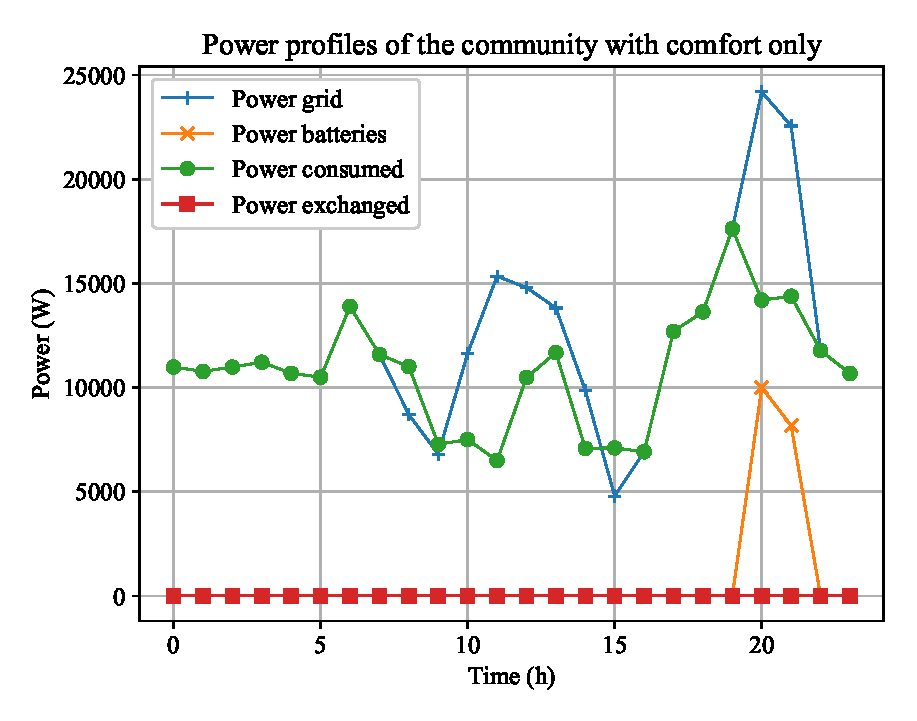
\includegraphics[width=\textwidth]{community_profiles/community_comfort_only_power_profiles.eps}
        \caption{Sociological profile [0, 0, 1]}
    \end{subfigure}
    \caption{Operation of the community with different sociological profiles.}
    \label{fig:diff_profiles}
\end{figure}



So now we will plot the Pareto front of the community by optimizing the community with different sociological profiles. To be able to compare efficiently the values in the Pareto front, it is plotted with the normalized values as explained in \ref{objective_function}. Figure \ref{fig:pareto_front} shows the 3D Pareto front of the community with the different sociological profiles. To understand better, we can also plot the 2D projections \ref{fig:pareto_front_2d}.

\begin{figure}[h]
    \centering
    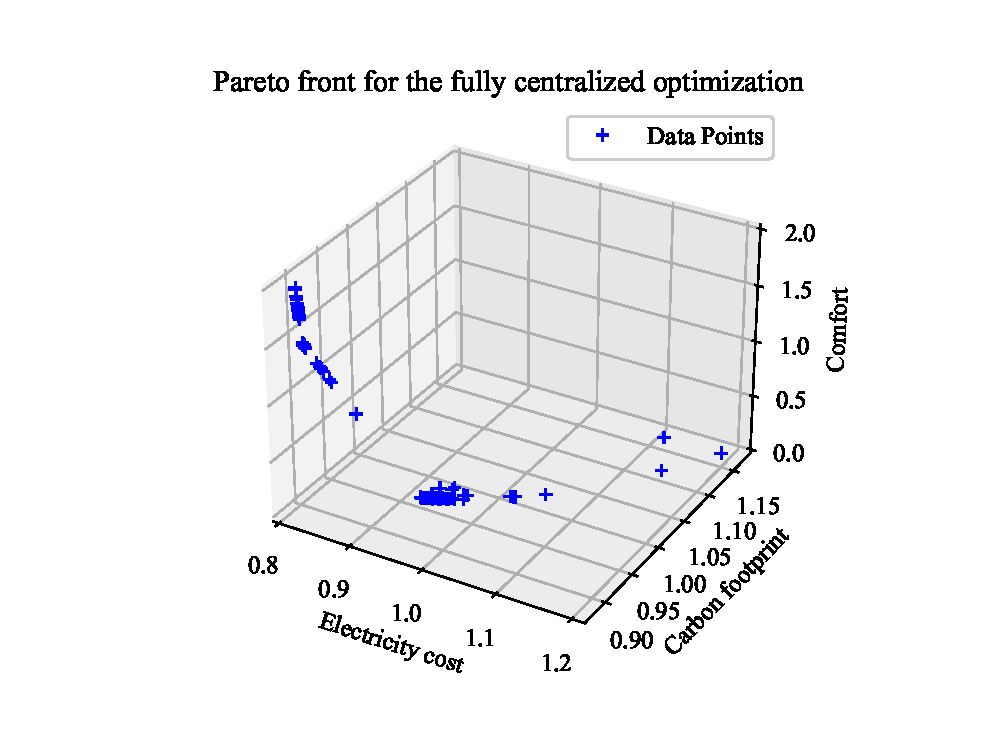
\includegraphics[width=0.8\textwidth]{commu_pareto_front.eps}
    \caption{3D Pareto front of the community with different sociological profiles.}
    \label{fig:pareto_front}
\end{figure}

\begin{figure}[h]
    \centering
    \begin{subfigure}[b]{0.32\textwidth}
        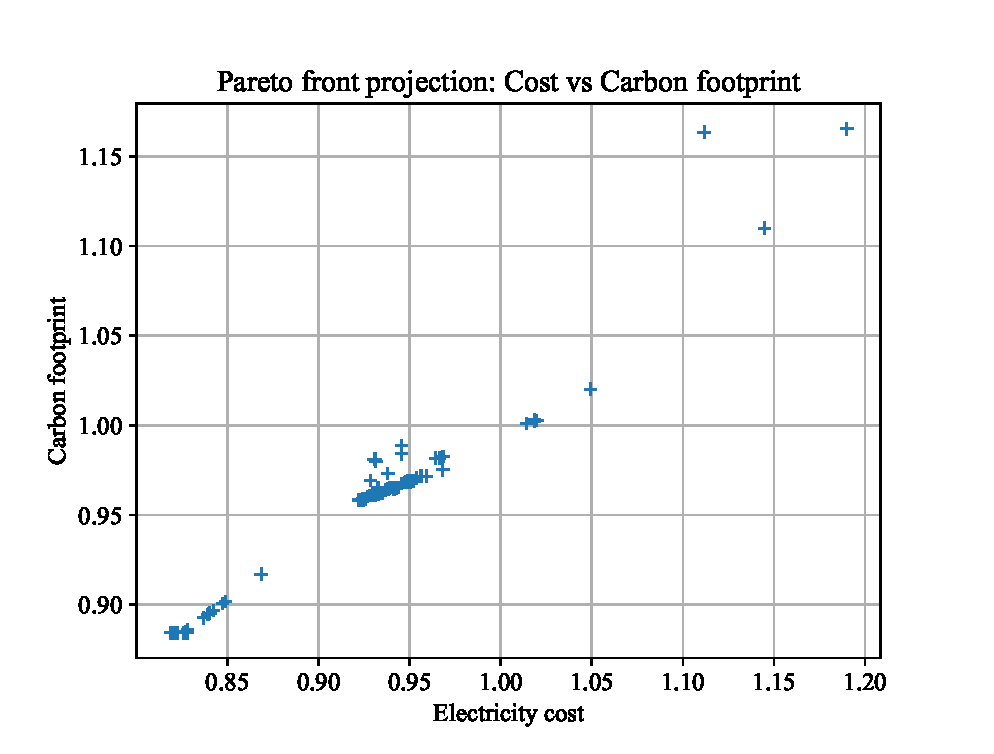
\includegraphics[width=\textwidth]{commu_pareto_front_cost_enviro.eps}
        \caption{Economic vs Environmental}
    \end{subfigure}
    \begin{subfigure}[b]{0.32\textwidth}
        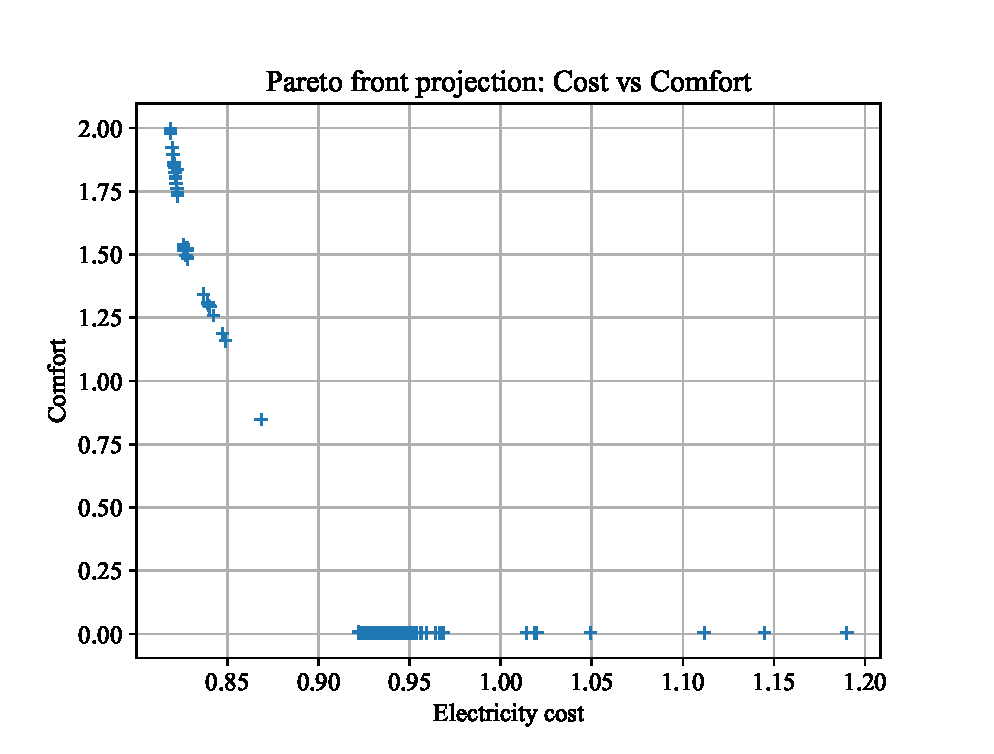
\includegraphics[width=\textwidth]{commu_pareto_front_cost_comfort.eps}
        \caption{Economic vs Comfort}
    \end{subfigure}
    \begin{subfigure}[b]{0.32\textwidth}
        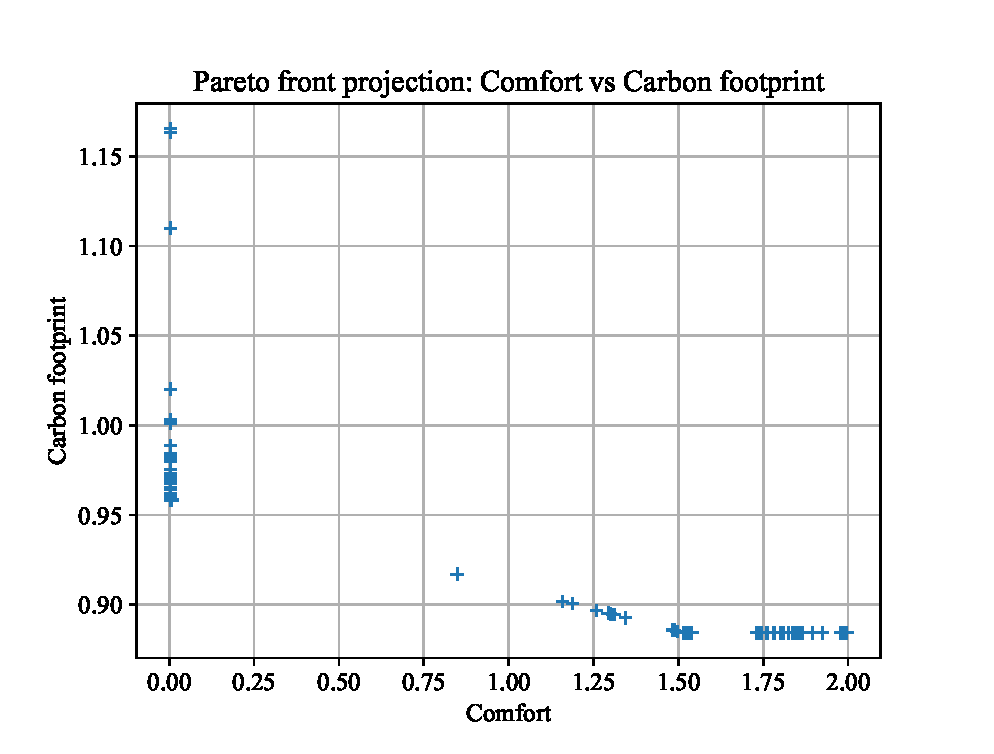
\includegraphics[width=\textwidth]{commu_pareto_front_comfort_enviro.eps}
        \caption{Comfort vs Environmental}
    \end{subfigure}
    \caption{2D projections of the Pareto front of the community with different sociological profiles.}
    \label{fig:pareto_front_2d}
\end{figure}

As we could have imagined while defining the objective function, there is a strong correlation between optimizing the environmental cost and the economic cost. Indeed, for both of them the cost is lower when we maximize the self consumption of the community. So the analysis between the comfort and the economic cost will be the same as between the comfort and the environmental cost. 

In the model, there is a minimum and a maximum comfort possible. The interesting part of the curve is thus the one where the comfort value is not yet at its maximum. And we can see that there is a clear trade-off between the comfort and the economic/environmental cost. The minimum economic cost for a comfort cost of 0 is around 0.92, while the minimum economic cost is around 0.82. Meaning a decrease of 11\%. The value is the same for the environmental cost. Of course this value depends a lot on the bounds we set, but the slopes of the curve can give us good insight on this trade-off. Another important point is that here the sociological profile of the community is computed as the average of the sociological profile of the members. So the trade-off to find will be between every member of the community.

Maybe a model involving the dimensioning of the production and storage capacities of the community would be more interesting for studying the Pareto Front as we should have more complex interactions between the price and the environmental cost. The model developed here could be improved for this by adding some variables and constraints.

\subsection{Gain allocation}

Now that we have seen the behavior of this community model, we will explore the gain allocation. For this, we will define some profiles for the members of the community as shown in \ref{tab:profiles}. They have been built in order to have a good variety of profiles in the community. The profile of the community is computed as the average of the profiles of the members. 

\begin{table}[h]
    \centering
    \begin{tabular}{|c|c|c|c|}
        \hline
        Member & Economic & Environmental & Comfort \\ \hline
        0      & 0.4  & 0.1  & 0.5     \\ \hline
        1      & 0.5  & 0.2  & 0.3     \\ \hline
        2      & 0.8  & 0.1  & 0.1     \\ \hline
        3      & 0.4  & 0.4  & 0.2     \\ \hline
        4      & 0.2  & 0.6  & 0.2     \\ \hline
        Community & 0.46 & 0.28 & 0.22    \\ \hline
    \end{tabular}
    \caption{Sociological profiles of the members of the community}
    \label{tab:profiles}
\end{table}

In this set-up, there is and economic gain of 15\% by participating in the community. In the figure \ref{fig:gain_allocation_radar}, we can see the comparison between each method.

\begin{figure}[h]
    \centering
    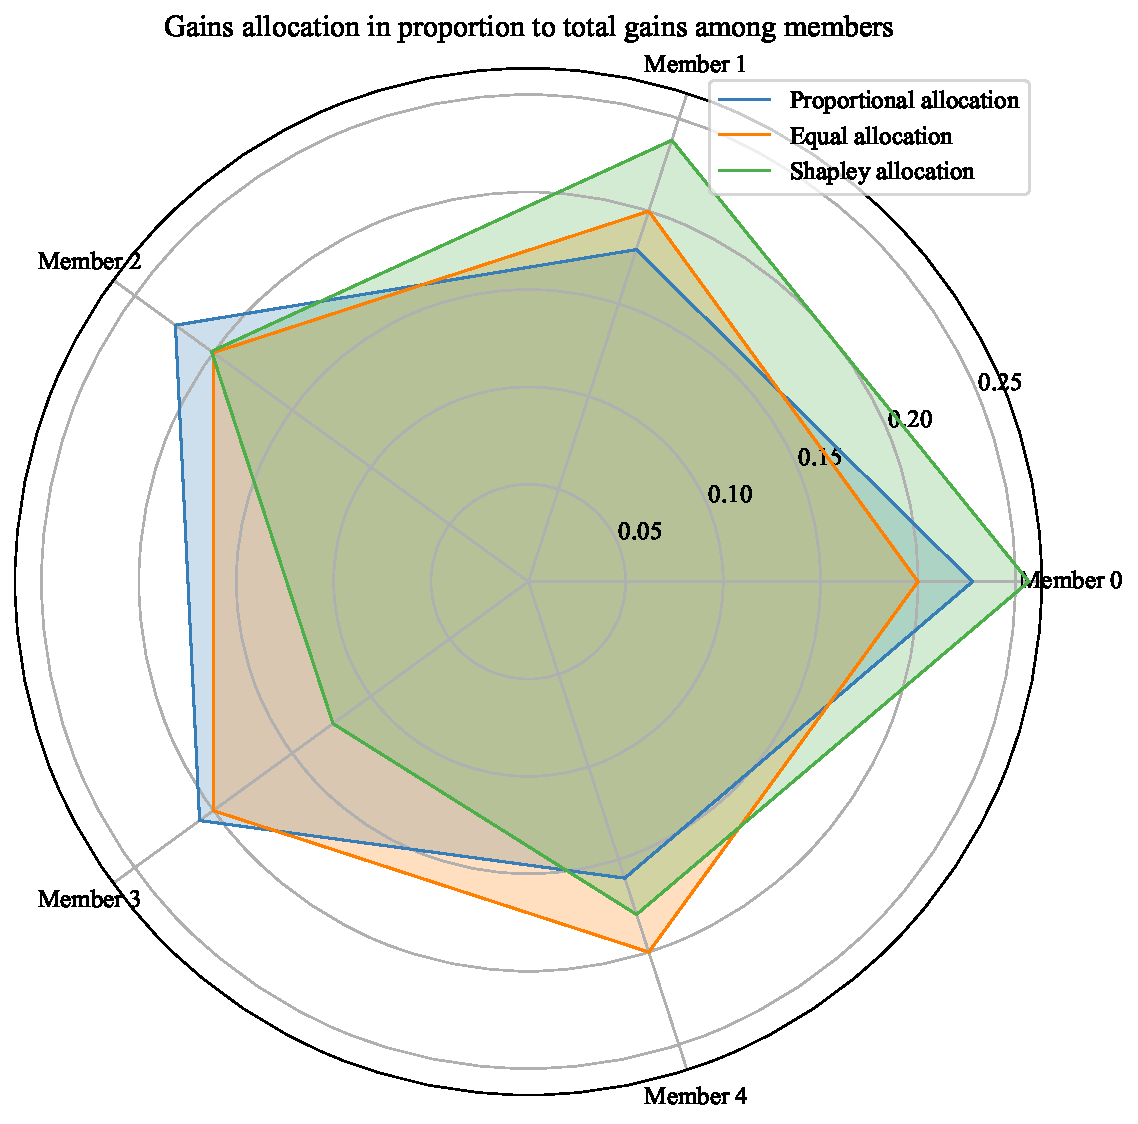
\includegraphics[width=0.5\textwidth]{gains_allocation/gains_allocation_proportional.pdf}
    \caption{Gains allocation in proportion to total gains among members.}
    \label{fig:gain_allocation_radar}
\end{figure}

Each method is not allocating the gain towards the same members. Here we can use the equal allocation as a reference in order to understand which members are favored by the different methods. The Shapley value gives more gain to members 0 and 1, a bit less to 2. Again a bit less to 4 and a lot less to 3. The proportional allocation is more equal by giving a bit more gain to 0, 2 and 3, and a bit less to 1 and 4.

One thing important to understand is that both methods have real mathematic arguments to be used. The Shapley value is a method that is based on the contribution of each member to the gain of the community, while the proportional allocation is a method that is based on the contribution of each member to the cost reduction of the community. But using one or the other result in differences in the gain allocation. To understand these results better we can compare the gain allocation with the resources of each member. Figure \ref{fig:gain_allocation_resources} shows each allocation compared to the installed production rate as well as the battery capacity rate and the consumption rate of each member.

\begin{figure}[!h]
    \centering
    \begin{subfigure}[b]{0.48\textwidth}
        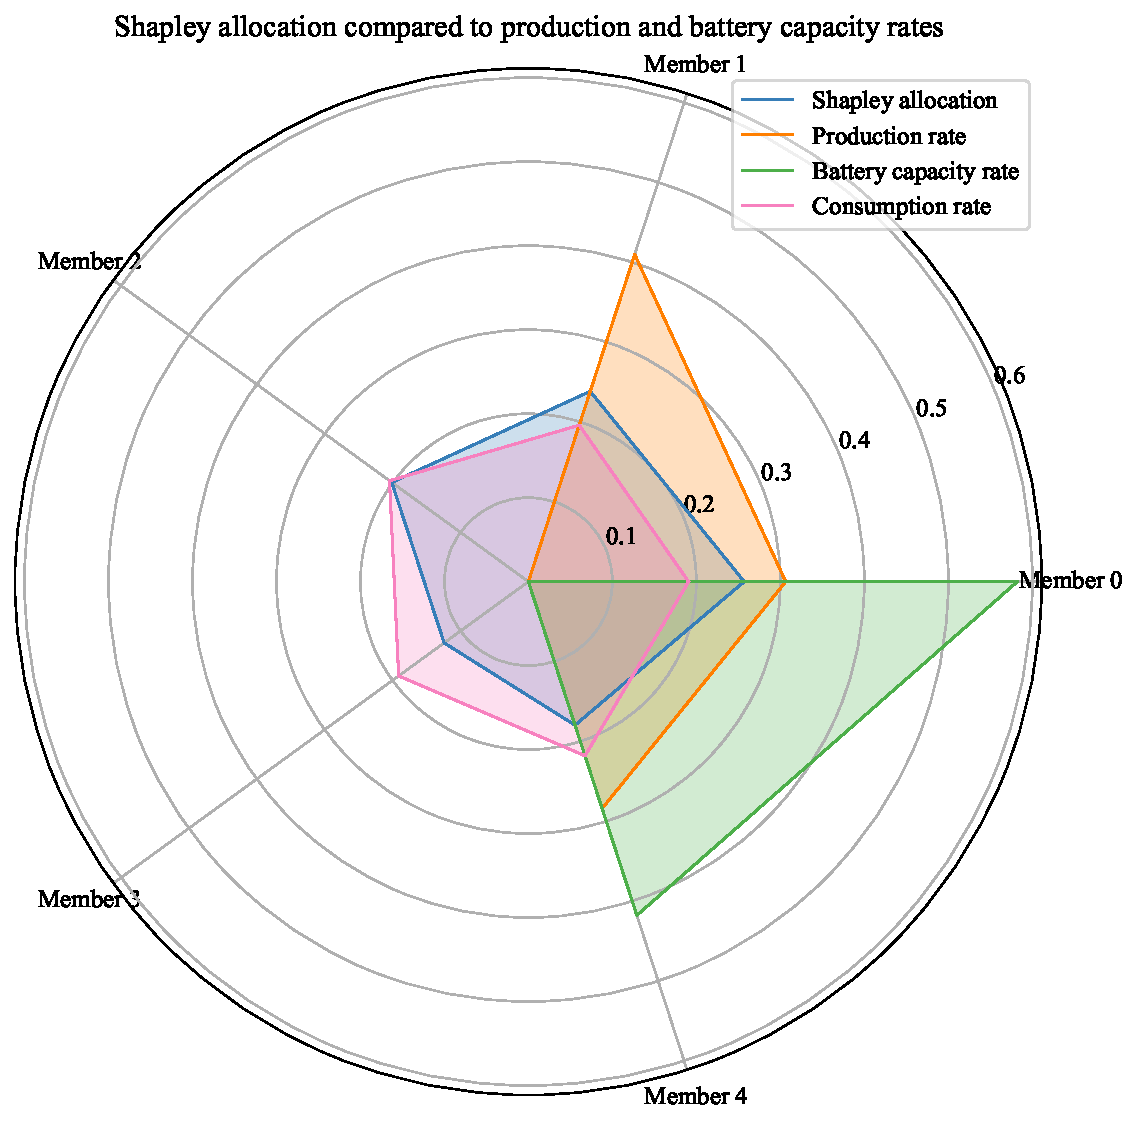
\includegraphics[width=\textwidth]{gains_allocation/shapley_vs_production_battery.pdf}
        \caption{Proportional allocation compared to the resources of each member.}
    \end{subfigure}
    \begin{subfigure}[b]{0.48\textwidth}
        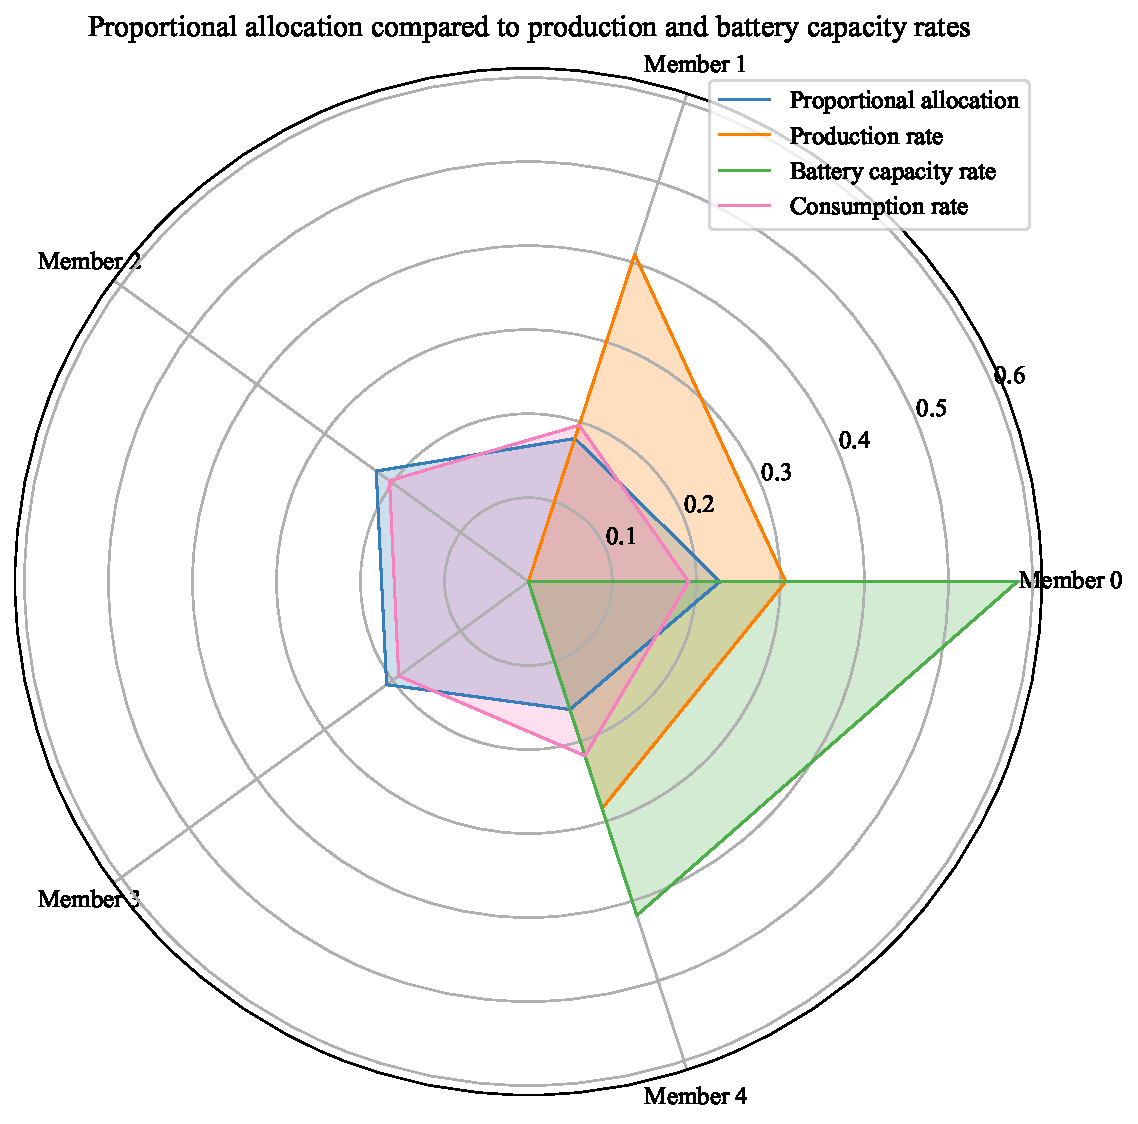
\includegraphics[width=\textwidth]{gains_allocation/proportional_vs_production_battery.pdf}
        \caption{Shapley allocation compared to the resources of each member.}
    \end{subfigure}
    \caption{Comparison of the gain allocation with the resources of each member.}
    \label{fig:gain_allocation_resources}
\end{figure}

The first thing we notice is that the consumption is almost equal for all members but member 4 which have a slightly higher consumption. Then as explained in the construction of the example, only member 0 and 4 have a battery capacity, and the one from 4 is available all day while the one from 0 is not available at midday. Finally, three members have a production, and the one from member 1 is higher than the two others. 

With this being said, the Shapley value works as expected in a meritocratic way by giving more gain to the members with solar production. But the consumption profile is also important. Indeed, we could think that member 4 would receive more as they have production and a battery storage. But having a higher consumption, they do not participate so much in reducing the objective cost of the community, and thus they do not receive a lot of gain. This behavior could bring some fairness problematics as the member 4 might receive less gain than member 2 for example, while he invested much more.

In the case of the proportional allocation, it seems hard to understand without understanding mathematically how the gain is computed. Indeed, two of the members receiving more gain than the others do not have any production. While, two of the members receiving less gain than the others have a production. This is because the gain is computed based on the cost reduction of the community as whole. So using this method that is supposed to reach Nash equilibrium, i.e. a state where no member can do better by changing its strategy while the other members keep their strategy unchanged, can lead to result that are not fair in a meritocratic way. It can be seen as a "max-min" fairness allocation function.

Of course the equal allocation is the most egalitarian one, it does not take into account the contribution of each member to the gain of the community at all. 



\bibliographystyle{IEEEtran}
\bibliography{references}

\end{document}